\documentclass[a4paper]{article}
\usepackage[T2A]{fontenc}
\usepackage[english,russian]{babel}
\usepackage{hyperref}
\usepackage{filecontents}
\hypersetup{
    colorlinks,
    citecolor=black,
    filecolor=black,
    linkcolor=black,
    urlcolor=blue
}
\usepackage{float}
\usepackage{subcaption}
\usepackage[utf8]{inputenc}
\usepackage[14pt]{extsizes}
\usepackage{physics} 
\usepackage{graphicx}
\graphicspath{{../misc/}}
\usepackage{setspace,amsmath}
\usepackage[left=30mm, right=15mm, top=20mm, bottom=20mm]{geometry} 
\usepackage[nottoc]{tocbibind}
\usepackage[backend=biber]{biblatex}
\addbibresource{lit.bib}
%%%%%%%%%%%%%%%%%%%%%%%%%%%%%%%%%%%%%
% \everymath{\displaystyle}
\DeclareMathSizes{12}{20}{14}{10}

\makeatletter 
\def\@makefnmark{\hbox{\@textsuperscript{\normalfont(\@thefnmark)}}}
\makeatother
% Отступ первого абзаца главы
\usepackage{indentfirst}

% Выставлять полуторные интервалы в тексте, но не вмешивается в подписи, таблицы и сноски
\usepackage{setspace}
% Установка нужного шрифта
\renewcommand{\rmdefault}{ftm}

% Красивые ссылки на литературу (конкретно, автоматическая сортировка и дефисы)

% Отключаем перенос
% \hyphenpenalty=10000 
% \usepackage{tocloft}  

% Устанавливаем шрифт 14 pt
\renewcommand{\tiny}{\fontsize{7}{8.4pt}\selectfont}
\renewcommand{\scriptsize}{\fontsize{9}{11pt}\selectfont}
\renewcommand{\footnotesize}{\fontsize{11}{13.6pt}\selectfont}
\renewcommand{\small}{\fontsize{12}{14.5pt}\selectfont}
\renewcommand{\normalsize}{\fontsize{14}{18pt}\selectfont}
\renewcommand{\large}{\fontsize{17}{20pt}\selectfont}
\renewcommand{\Large}{\fontsize{20}{25pt}\selectfont}

% \usepackage{utf8gost705u}
% \bibliographystyle{utf8gost705u}

\captionsetup[figure]{labelformat=parens, labelsep=period}
\captionsetup[table]{labelformat=parens, labelsep=period}

\begin{document} 

\begin{center}
    \hfill \break
    ФЕДЕРАЛЬНОЕ ГОСУДАРСТВЕННОЕ БЮДЖЕТНОЕ ОБРАЗОВАТЕЛЬНОЕ 

    УЧРЕЖДЕНИЕ ВЫСШЕГО ОБРАЗОВАНИЯ

    «МОСКОВСКИЙ ГОСУДАРСТВЕННЫЙ УНИВЕРСИТЕТ

    имени М.В.ЛОМОНОСОВА» 

    \hfill \break
    \normalsize{ФИЗИЧЕСКИЙ ФАКУЛЬТЕТ}\\
    \hfill \break
    \normalsize{КАФЕДРА ОБЩЕЙ ФИЗИКИ И МОЛЕКУЛЯРНОЙ ЭЛЕКТРОНИКИ}\\
    \hfill \break
    \normalsize{БАКАЛАВРСКАЯ РАБОТА}\\
    \hfill \break
    \large\textbf{«МОДЕЛИРОВАНИЕ РАСПОЗНАВАНИЯ ОБРАЗОВ НА ОСНОВЕ ИМПУЛЬСНЫХ НЕЙРОННЫХ СЕТЕЙ С КОНКУРЕНЦИЕЙ ЛОКАЛЬНЫХ РЕЦЕПТИВНЫХ ПОЛЕЙ»}\\

\end{center}

\begin{flushright}

    Выполнил студент

    406 группа

    Гафни Д.

    $\underset{\text{подпись студента}}{\underline{\hspace{0.3\textwidth}}}$

    \hfill\break

    Научный руководитель:

    н.с Королёва А.В.

    $\underset{\text{подпись научного руководителя}}{\underline{\hspace{0.3\textwidth}}}$
    
    \hfill\break
    
    Научный консультант:

    Дёмин В.А.

    $\underset{\text{подпись научного консультанта}}{\underline{\hspace{0.3\textwidth}}}$

\end{flushright}


Допущена к защите

Зав.кафедрой $\underset{\text{подпись зав.кафедрой}}{\underline{\hspace{0.3\textwidth}}}$
\hfill\break
\hfill\break
\begin{center}

Москва

\hfill\break
2020
\end{center}

\thispagestyle{empty}

\tableofcontents

\clearpage 

\addcontentsline{toc}{section}{Введение}
\section*{\centering{Введение}}
Импульсные (\textit{спайковые}) нейронные сети (СНС) являются перспективным нейроморфным алгоритмом, биологически корректно моделируя взаимодействия нейронов мозга. Наибольший интерес СНС представляют для решения задач в реальном времени (принятие решений, распознавание образов), так как могут быть реализованы на специализированном вычислительно- и энергоэффективном нейрочипе (например, на основе мемристоров) \cite{hardware1, hardware2}.

Стандартные методы обучения весов связей, применяющиеся в формальных нейронных сетях (метод обратного распространения ошибки) не представляется возможным применять к СНС из-за их дискретной и распределенной во времени природы. Таким образом, исследование алгоритмов обучения СНС представляется важной задачей.

\addcontentsline{toc}{subsection}{Мотивация}
\subsection*{\centering{Мотивация}}
Современные формальные нейронные сети отлично справляются со многими задачами машинного обучения \cite{pmlr-v28-wan13}. Однако их обучение --- трудоемкий процесс, требующий больших вычислительных ресурсов. Обычно обучение ведется на десятках и сотнях тысяч примеров и может занимать месяцы. Как само обучение, так и последующее применение формальных нейросетевых алгоритмов далеки от эффективности. Это связано как с физически раздельным хранением значений весов и активаций нейронов, так и с самими вычислениями, которые носят тензорный характер. Современные процессоры не оптимизированы для подобных вычислений. Гораздо лучше процессоров для этих задач подходят GPU --- архитектуры, изначально созданные для работы с компьютерной графикой, а потому лучше подходящие для тензорных вычислений, однако и они не дают желаемого результата. Число параметров в современных формальных нейронных сетях может достигать сотен миллионов \cite{ManyParams}.

\addcontentsline{toc}{subsection}{Постановка задачи}
\subsection*{\centering{Постановка задачи}}
В данной работе:

\begin{enumerate}
\item Изучается влияние обучения связей конкуренции \cite{MaxActiv1, MaxActiv2, hardware_survey} между нейронами на точность распознавания образов в задаче классификации рукописных изображений цифр из датасета MNIST \cite{MNIST} при обучении без учителя для архитектуры локально соединенной сети (Locally Connected Spiking Neural Network, LCSNN) \cite{saunders2019locally}.

\item Проводится сравнение этой архитектуры со сверточной сетью (Convolution Spiking Neural Network, CSNN) и полносвязной сетью (Fully Connected Spiking Neural Network, FCSNN).

\end{enumerate}

\clearpage 

\section{\centering{Спайковые нейронные сети}}
Спайковая нейронная сеть --- модель нейронной сети, элементами которой являются  отдельные \textit{нейроны} и \textit{связи} (соответствующие синапсам реальных нейронов) между ними. Каждый нейрон имеет свой виртуальный \textit{потенциал}, а каждая связь имеет некоторый \textit{вес}. Нейроны обмениваются дискретными электрическими сигналами (\textit{спайками}), имеющими очень короткую ($ \approx ~1$ мс) длительность. Входящий спайк носит название \textit{пре-спайка}, а исходящий --- \textit{пост-спайка}.  Влияние пре-спайков на потенциал нейрона определяется значением веса межнейронной связи. При накоплении потенциала, превышающего определенный \textit{порог активации}, нейрон сам испускает пост-спайк, а после сбрасывает свое напряжение до значения \textit{потенциала сброса}. При запуске сети активность некоторых входных нейронов задается определенным образом, после чего проводится симуляция на протяжении некоторого времени ($\approx ~250$ мс), много большего длительности спайка.

\subsection{\centering{Преимущества спайковых нейронных сетей}}
Спайковые нейронные сети имеют ряд преимуществ перед формальными нейронными сетями.

\begin{itemize}
\item Для обучения спайковых нейронных сетей могут применять локальные алгоритмы, которые используют для обновления веса каждой связи лишь информацию, источником которой являются нейроны, которые эта связь соединяет. Напротив, при обучении формальных нейронных сетей для обновления веса каждой связи используется информация о всех связях, стоящих между этой связью и выходом сети. Таким образом, сами по себе алгоритмы обучения спайковых нейронных сетей являются более эффективными, чем алгоритмы обучения формальных нейронных сетей.
\item Более того, эти алгоритмы используют обучение без учителя (unsupervised learning), для которого не требуется ручной разметки данных.
\item Спайковые нейронные сети могут быть реализованы на специализированном сверхэффективном нейроморфном процессоре. Такая реализация вместе с чисто алгоритмическим преимуществом спайковых нейронных сетей дает еще больший выигрыш в производительности и энергоэффективности \cite{hardware1, hardware2}. 
\item Спайковые нейронные сети биологически корректно моделируют взаимодействия нейронов, что может использоваться для биологических симуляций нервной системы.
\end{itemize}

\subsection{\centering{Модели нейронов спайковой нейронной сети}}
Реальный нейрон мозга является очень сложным объектом, поведение которого до сих пор не до конца изучено. Для спайковых нейронных сетей используются упрощенные модели нейронов \cite{neuronmodels}. Перечислим некоторые из них.

\subsubsection{\centering{Пороговый нейрон}}
Это наиболее упрощенная модель нейрона. В каждый момент времени нейрон осуществляет следующие действия:

\begin{enumerate}
 \item Суммирует входящие сигналы

\begin{equation} \label{eq:thresh}
v(t) = v_{reset} + R \cdot \sum_{i=1}^n {w_i I_i} \text{, где}
\end{equation}

$v(t)$ --- потенциал нейрона, $v_{reset}$ --- уровень сброса, $w_i$ --- вес $i$-ой связи, $I_i$ --- <<ток>> $i$-ой связи, принимающий значение 1, если от нее есть спайк и 0, если его нет, а $R$ --- размерный коэффициент, численно равный 1.

\item Осуществляет сравнение $v(t)$ с $v_{thresh}$ --- значением порога активации. Если потенциал превосходит порог активации, то нейрон испускает спайк и сбрасывает свой потенциал до $v_{reset}$. Если потенциал не превосходит порог активации, то нейрон просто сбрасывает свой потенциал до значения $v_{reset}$.
\end{enumerate}

\begin{center}
\begin{figure}[H] 
 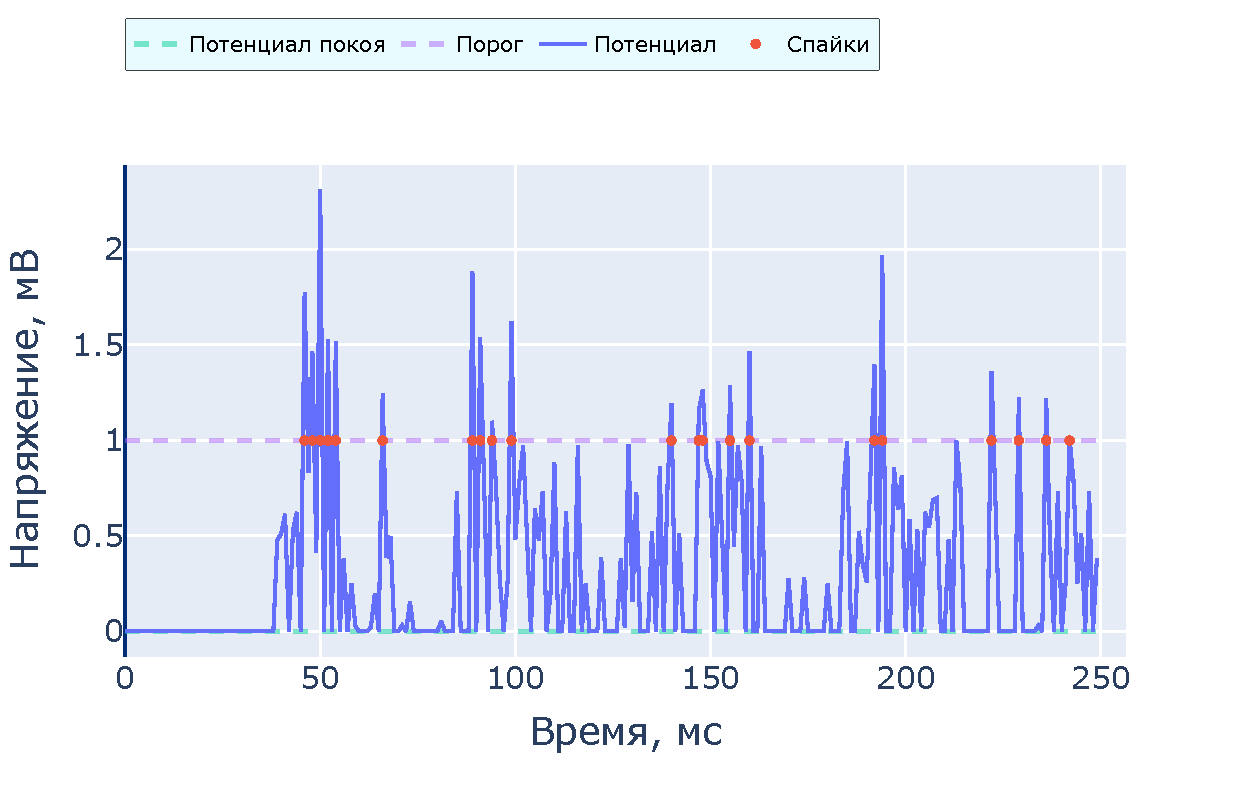
\includegraphics[width=\textwidth,keepaspectratio=true]{model_thresh_ru.pdf}
 \caption{Типичная зависимость потенциала порогового нейрона от времени. Красными точками отмечены спайки нейрона. В каждый момент времени потенциал нейрона равен взвешенной сумме входящих спайков.}
\end{figure}
\end{center}

\subsubsection{\centering{Пороговый интегратор}}
Это немного усложненная модель нейрона (Integrate-and-Fire, IF), в которой нейрон приобретает способность накапливать входящие сигналы во времени. В каждый момент времени нейрон осуществляет следующие действия:

\begin{enumerate}
 \item суммирует входящий сигнал

\begin{equation} \label{eq:if}
v(t) = v_{reset} + R \cdot \sum_{i=1}^n {w_i I_i} + R \cdot I(t) \text{, где}
\end{equation}

$I(t)$ --- накопленный к этому моменту ток от входящих спайков, а остальные переменные обозначены в выражении \ref{eq:thresh}.

\item осуществляет сравнение $v(t)$ с $v_{thresh}$ --- значением порога активации. Если потенциал превосходит порог активации, то нейрон испускает спайк и сбрасывает свой потенциал до значения $v_{reset}$, а также сбрасывает $I(t)$ до 0, после чего наступает короткий период рефрактерности, при котором на протяжении времени $t_{refract}$ потенциал нейрона остается на уровне $v_{reset}$. Если же потенциал не превосходит порога активации, то нейрон просто обновляет значение $I(t)$.
\end{enumerate}

\begin{center}
\begin{figure}[H] 
 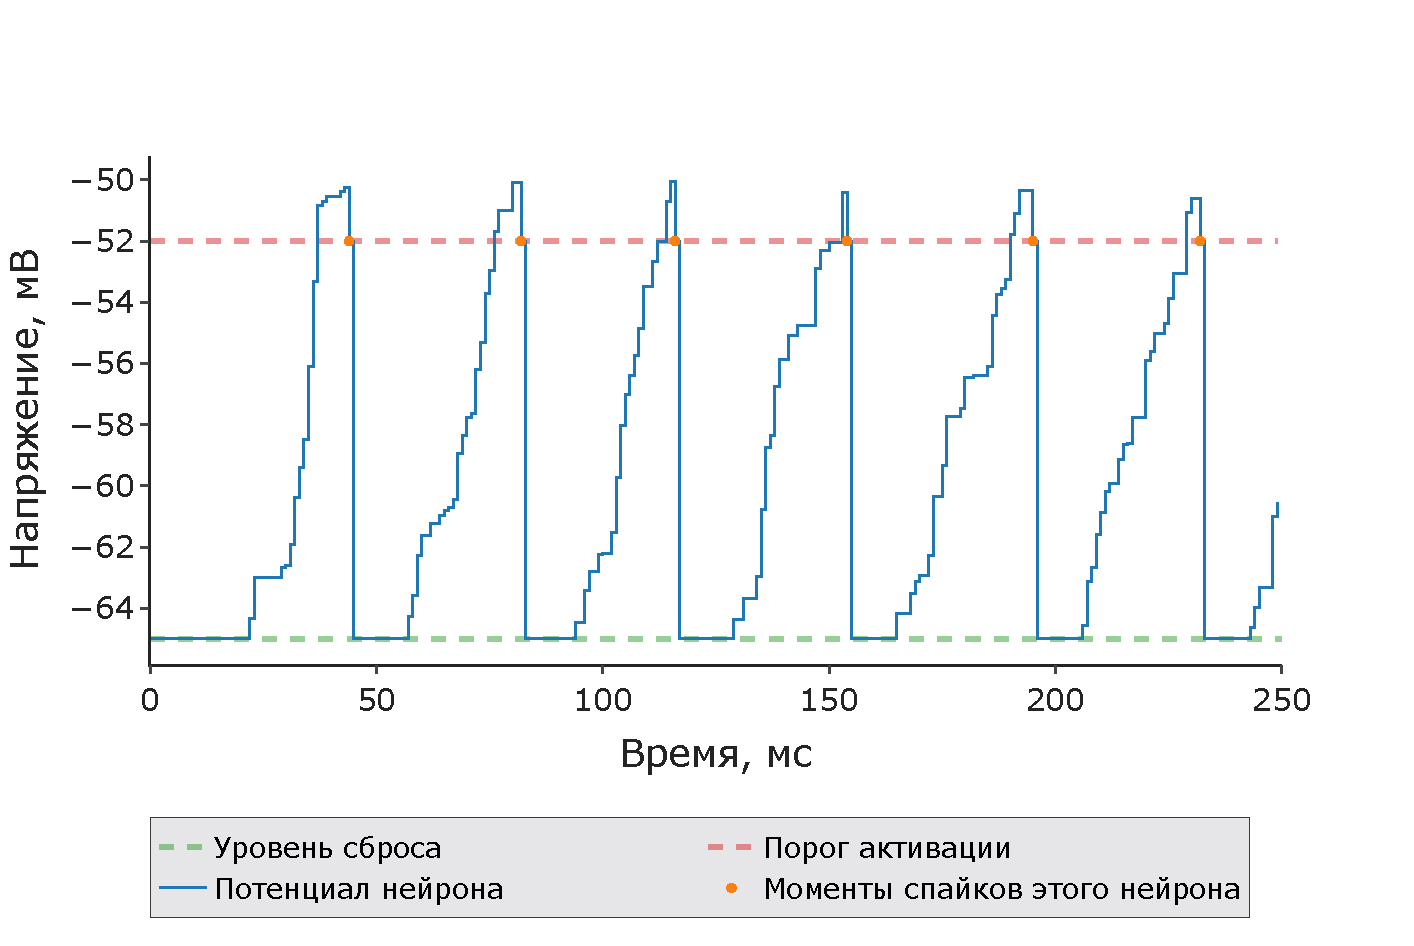
\includegraphics[width=\textwidth,keepaspectratio=true]{model_if_ru.pdf}
 \caption{Типичная зависимость потенциала порогового интегратора от времени. Красными точками отмечены спайки нейрона. В отличие от предыдущей модели, потенциал накапливается, пока не достигнет порога активации.}
\end{figure}
\end{center} 

\subsubsection{\centering{Пороговый интегратор с утечкой}}
Это еще более усложненная модель нейрона (Leaky-Integrate-and-Fire, LIF), в которой его потенциал приобретает <<утечку>>, то есть стремится с течением времени сравняться с \textit{уровнем релаксации} $v_{rest}$. В этой модели динамика потенциала задается следующим уравнением:

\begin{equation} \label{eq:lif}
 \tau_v \dv{v(t)}{t} = -v(t) + v_{rest} + I(t) \cdot R \text{, где}
\end{equation} где $\tau_v$ --- временная константа симуляции, остальные переменные обозначены в выражениях \ref{eq:if} и \ref{eq:thresh}.

После испускания каждого спайка наступает короткий период рефрактерности, при котором на протяжении времени $t_{refract}$ потенциал нейрона остается на уровне $v_{reset}$.

Таким образом, потенциал нейрона сам по себе стремится вернуться в состояние релаксации, так как если $I(t) = 0$ (нет входящих спайков) и $v(t) = v_{rest}$, то производная $\dv{v(t)}{t} = 0$, то есть потенциал нейрона будет оставаться постоянным на уровне $v_{rest}$. 

\begin{center}
\begin{figure}[H] 
 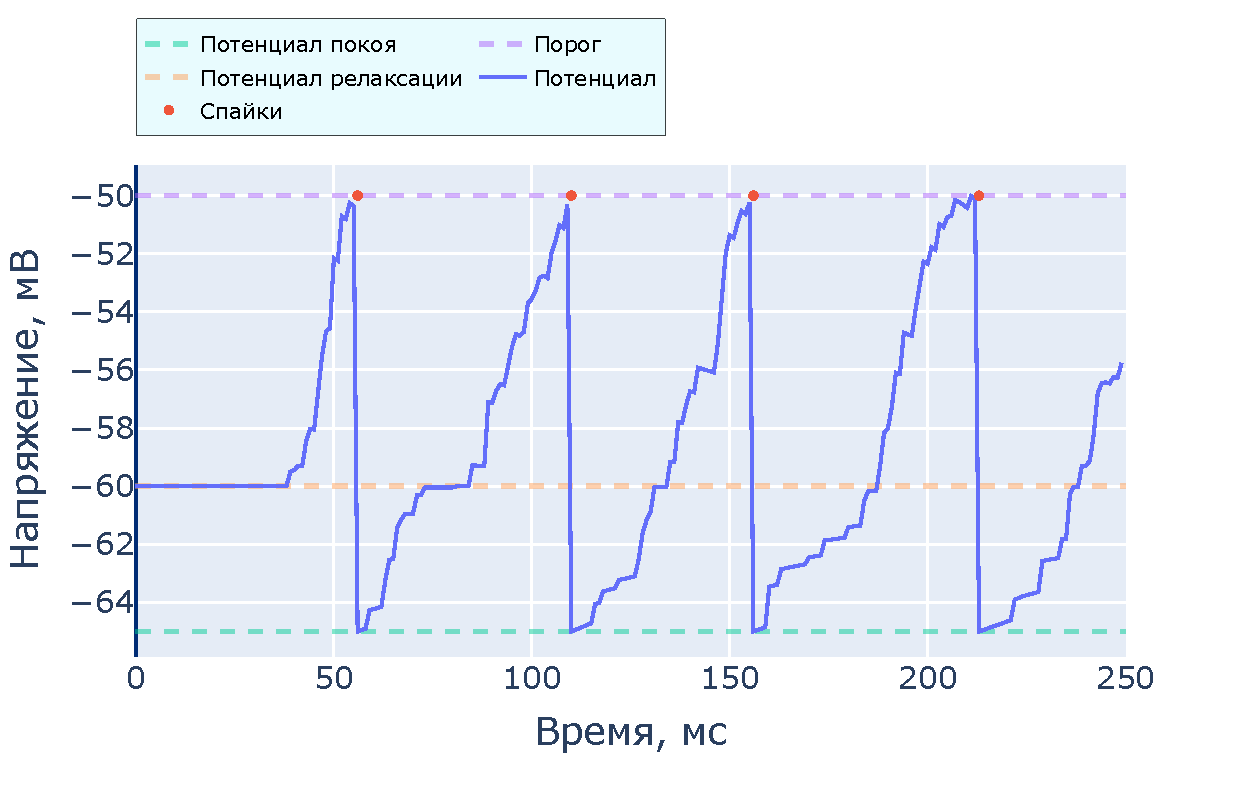
\includegraphics[width=\textwidth,keepaspectratio=true]{model_lif_ru.pdf}
 \caption{Типичная зависимость потенциала порогового интегратора с утечкой от времени. Красными точками отмечены спайки нейрона. Видно, что потенциал нейрона сам по себе стремится к значению потенциала релаксации, чего не происходит в предыдущей модели.}
\end{figure}
\end{center}

\subsubsection{\centering{Пороговый интегратор с утечкой и адаптивным порогом}}
В данной работе используется именно эта модель (Adaptive Leaky Integrate-and-Fire, A-LIF), самая сложная из представленных. В этой модели динамика потенциала задается таким же уравнением, как и у LIF нейрона:

\begin{equation} \label{eq:alif}
 \tau_v \dv{v(t)}{t} = -v(t) + v_{rest} + I(t) \cdot R \text{,}
\end{equation} где $I(t)$ --- ток, накопившийся в нейроне к моменту времени $t$, $v_{rest}$ --- уровень релаксации, $\tau_v$ --- временная константа симуляции.\\ 

Таким образом, потенциал нейрона сам по себе стремится вернуться в состояние релаксации, так как если $I(t) = 0$ (нет входящих спайков) и $v(t) = v_{rest}$, то производная $\dv{v(t)}{t} = 0$, то есть потенциал нейрона будет оставаться постоянным на уровне $v_{rest}$. 

Порог активации $v_{thresh}$ у ALIF нейрона не является константой, а немного повышается при каждом спайке, релаксируя затем к своему начальному значению $\theta_o$. Динамика порога активации задается следующими уравнениями:
\begin{equation} 
 v_{thresh} = \theta_0 + \theta(t) \text{,}
\end{equation} где $\theta_0$ --- начальный порог активации, $\theta(t)$ --- адаптивная добавка, которая вычисляется из условия\\

\begin{equation}
 \tau_v \dv{\theta(t)}{t} = -\theta(t)
\end{equation}\\

Также после испускания каждого спайка адаптивная добавка $\theta(t)$ повышается на $\theta_{plus}$.

Таким образом, порог активации нейрона сам по себе стремится вернуться к начальному значению, так как при $\theta(t) = \theta_0$, то производная $\dv{\theta(t)}{t} = 0$, то есть порог активации нейрона будет оставаться постоянным на уровне $\theta_0$.\\

После испускания каждого спайка наступает короткий период рефрактерности, при котором на протяжении времени $t_{refract}$ потенциал нейрона остается на уровне $v_{reset}$.

\begin{center}
\begin{figure}[H]
 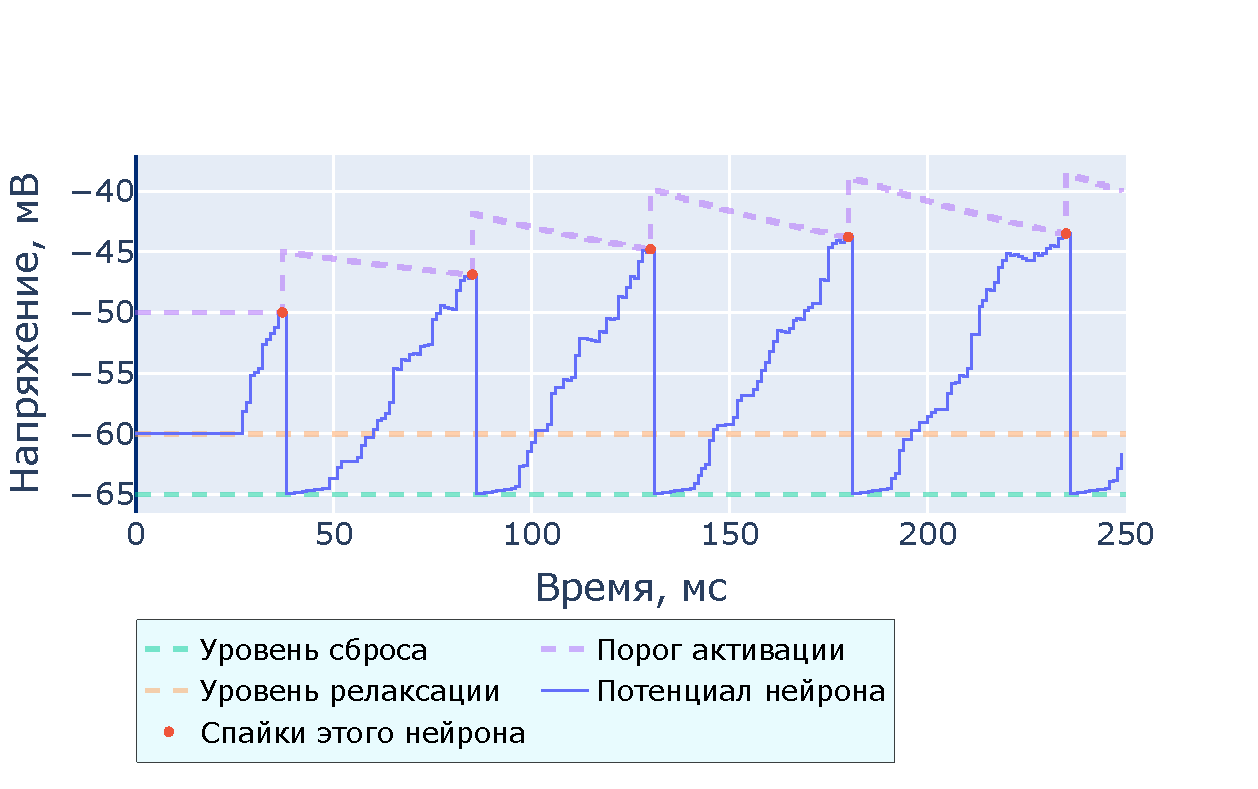
\includegraphics[width=\textwidth,keepaspectratio=true]{model_alif_ru.pdf}
 \caption{Типичная зависимость потенциала порогового интегратора с утечкой и адаптивным порогом от времени. Красными точками отмечены спайки нейрона. Видны скачки порога активации после испускания спайков и его постепенное возвращение к исходному уровню.\\
 \textit{Примечание: здесь исключительно для наглядности используется такое большое значение $\theta_{plus}$, в реальных экспериментах его влияние менее значительно.}}
\end{figure} 
\end{center}

\subsection{\centering{Архитектуры спайковых нейронных сетей}}
Современные архитектуры формальных нейронных сетей могут переноситься на спайковые нейронные сети. При этом для увеличения эффективности разделения нейронов по признакам используются связи конкуренции (Рис. \ref{competition-training-importance}). 

\subsubsection{\centering{Полносвязная сеть}}
В полносвязной сети два слоя $X$ и $Y$ имеют связи между всеми парами нейронов.

Число нейронов $Y$ слоя и его структура задается произвольно. Число параметров (весов) такой сети равно $\frac{XY}{2}$.

\subsubsection{\centering{Сверточная сеть}}
В сверточной сети для построение связей и формирования $Y$ слоя применяется операция \textit{свертки}. Пусть есть $X$ слой нейронов $N \times M$. Операция свертки определяется 4 параметрами: размером \textit{ядра} свертки ($k_1$, $k_2$) и \textit{шагом} свертки ($s_1$, $s_2$).

\begin{figure}[H]
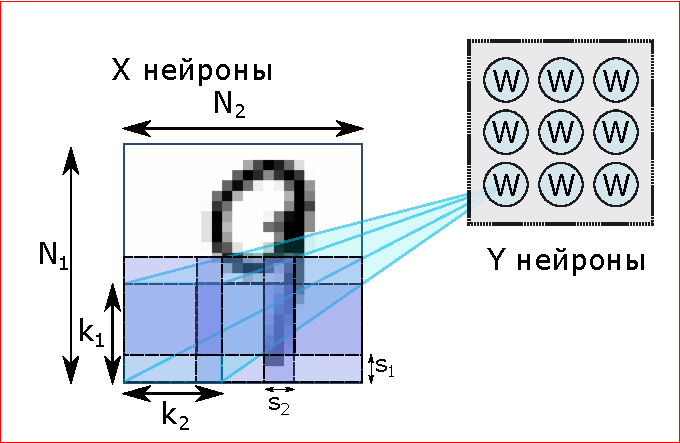
\includegraphics[,
 width=\textwidth,keepaspectratio=true]{convolution.pdf}
    \caption{Свертка}
\end{figure}

$Y$ нейроны также называются \textit{сверточным} слоем. Все они имеют общие (численно совпадающие) веса $W$ связей $XY$ размерности ($k_1 \times k_2$). Отличаются нейроны положением области $X$ слоя, с которой имеются связи.

Размерность $Y$ слоя равна
($\frac{N_1 - k_1 - 2}{s_1}$, $\frac{N_2 - k_2 - 2}{s_2}$). Число параметров свертки равно $k_1 \cdot k_2$. 

Заметим, что свертки могут применяться над предыдущим слоем любой размерности. Здесь была описана 2-D свертка, принцип ее работы аналогично переносится и на N-D. 

В дальнейшем ядро свертки $k_{1} \times k_{2} $ будем также называть синонимами --- \textit{<<область видимости>>}, \textit{<<рецептивное поле>>}. Также в этой работе для упрощения подбора оптимальных параметров используются только квадратные свертки, т.е. $k_{1} = k_{2} \equiv k$, а $s_{1} = s_{2} \equiv s$. Все сети в этой работе имеют шаг $s = 2$.

\subsubsection{\centering{Локально соединенная сеть}}
Локально соединенная архитектура совпадает со сверточной с тем единственным отличием, что веса $Y$ нейронов для нее не являются общими, то есть каждый $Y$ нейрон имеет свои уникальные веса связей $XY$.

\begin{figure}[H]
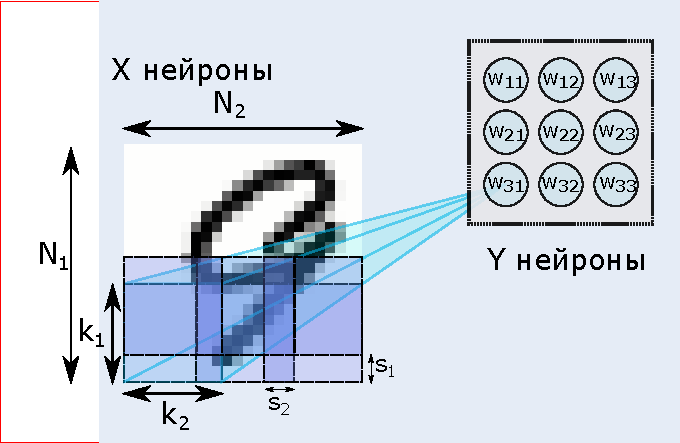
\includegraphics[,
 width=\textwidth,keepaspectratio=true]{local_connection.pdf}
    \caption{Локальное соединение}
\end{figure}

Размерность $Y$ слоя для локально соединенной сети равна ($\frac{N_1 - k_1 - 2}{s_1}$, $\frac{N_2 - k_2 - 2}{s_2}$), число связей равно $\frac{N_1 - k_1 - 2}{s_1} \cdot \frac{N_2 - k_2 - 2}{s_2} \cdot k_1 \cdot k_2$.

Как и свертка, локально соединенный слой может быть аналогичным образом основан на слое любой размерности. Для локально соединенных сетей также используются только квадратные свертки, т.е. $k_{1} = k_{2} \equiv k$, а $s_{1} = s_{2} \equiv s$. Все сети в этой работе имеют шаг $s = 2$.

\subsection{\centering{Алгоритмы обучения спайковых нейронных сетей}}
Процесс нахождения оптимальных значений весов связей сети называется обучением. Обучением может вестись как с учителем --- если алгоритме обучения используется информация об истинных значениях, предсказываемых сетью --- так и без учителя. Преимущество первого класса алгоритмов обучения заключается в как правило лучших результатах, а недостаток --- в необходимости предварительной разметки обучающей выборки человеком, что не всегда представляется возможным. В свою очередь, обучения без учителя может давать немного худшие результаты в зависимости от задачи, однако не требует разметки данных, что часто позволяет подготавливать большие объемы обучающей выборки, чем при обучении без учителя. В данной работе для обучения используется правило STDP (Spike Timing Dependent Plasticity).

\subsubsection{\centering{STDP}}
STDP --- биологически инспирированное правило обучения без учителя \cite{STDP}. При получении пре-спайка и испускании пост-спайка вес $w$ связи, по которой пришел пре-спайк, увеличивается на $\Delta w$, где
\begin{equation} 
\Delta w =
 \begin{cases}
 A_+ \cdot e^{- \frac{t_{pre} - t_{post}}{\tau_+}}, t_{pre} - t_{post} > 0\\
 A_- \cdot e^{- \frac{t_{pre} - t_{post}}{\tau_-}}, t_{pre} - t_{post} < 0
 \end{cases}
\end{equation}

Заметим, что

$$
\begin{cases}
 A_{+} > 0\\
 A_{-} < 0
\end{cases}
$$

\begin{figure}[H] \label{fig:STDP} 
\begin{center}
 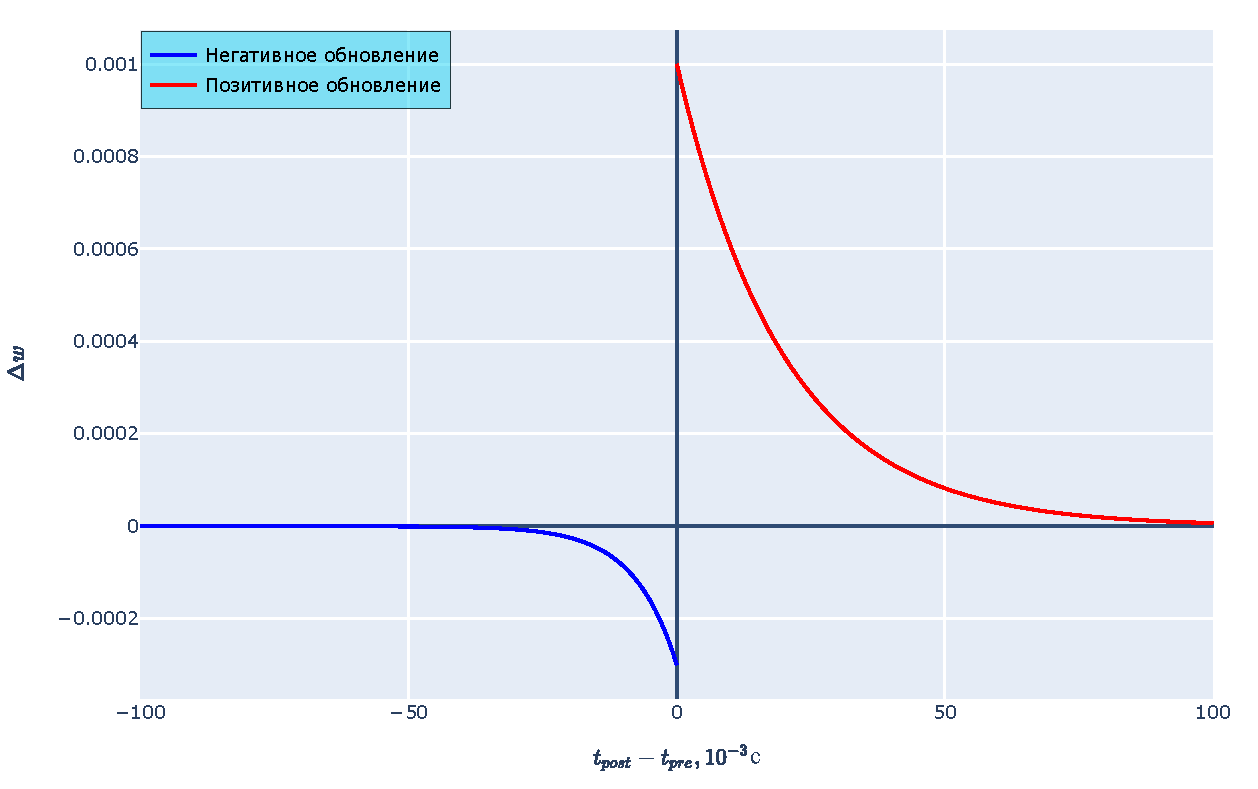
\includegraphics[,
 width=\textwidth,keepaspectratio=true]{STDP_ru.pdf}
 
 \caption{Правило STDP. График зависимости изменения веса от разности времени регистрации пост- и пре- спайков.}
\end{center}
\end{figure}

Таким образом, в процессе обучения у каждого нейрона увеличивается вес связей, по которым систематически пре-спайк приходит перед излучением пост-спайка, и наоборот, вес уменьшается у тех связей, для которых такой закономерности не наблюдается. После такого обучения нейрон начинает активнее реагировать на пре-спайки от нейронов, соединенных с ним связями с большими весами, а значит, начинает сам испускать пост-спайк, если в короткий промежуток времени эти нейроны будут активны одновременно.  Этим он объединяет их активность, посылая пост-спайк дальше по сети.


\subsubsection{\centering{anti-STDP} \label{sec:anti-STDP}}
anti-STDP является правилом обучения, обратным к STDP.

\begin{equation} 
\Delta w =
 \begin{cases}
 A_+ \cdot e^{- \frac{t_{pre} - t_{post}}{\tau_+}}, t_{pre} - t_{post} > 0\\
 A_- \cdot e^{- \frac{t_{pre} - t_{post}}{\tau_-}}, t_{pre} - t_{post} < 0
 \end{cases}
\end{equation}

$$
\begin{cases}
 A_{+} < 0\\
 A_{-} > 0
\end{cases}
$$

\begin{figure}[H] \label{fig:anti-STDP} 
\begin{center}
 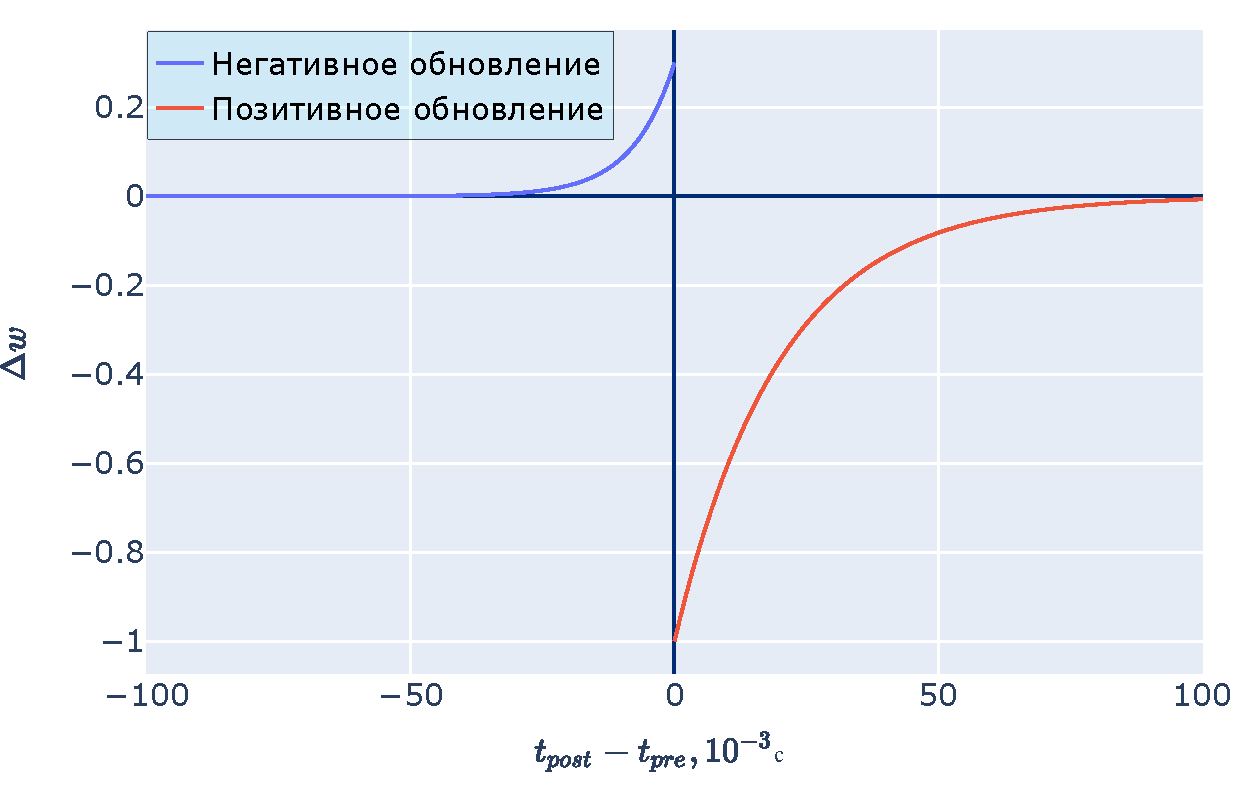
\includegraphics[,
 width=\textwidth,keepaspectratio=true]{anti-STDP_ru.pdf}
 
 \caption{Правило anti-STDP. График зависимости изменения веса от разности времени регистрации пост- и пре- спайков.}
\end{center}
\end{figure}

Таким образом, в процессе обучения вес связей между нейронами, активность которых корреллирует, уменьшается. Это правило используется для обучения связей конкуренции.

\subsection{\centering{Современные аппаратные реализации спайковых нейронных сетей}}
На сегодняшний день создано несколько нейроморфных процессоров для аппаратной реализации спайковых нейронных сетей. Рассмотрим их. В таблице также указаны аналогичные параметры человеческого мозга.

\begin{table}[h]
 \caption {Сравнительная таблице аппаратных реализаций спайковых нейронных сетей. Указано энергопотребление при решении типичной задачи машинного обучения.}
 \begin{center}
  \begin{tabular}{|c|c|c|c|}
  \hline
  {Название} & {Нейроны} & {Синапсы} & {Энергопотребление, мВт}\\
  \hline
  {Мозг человека} & {$\approx 100 \cdot 10^9$} & {$\approx 1 \cdot 10^{14}$} & {20000}\\
  \hline
  {TrueNorth \cite{TrueNorth}} & {$1 \cdot 10^6$} & {$256 \cdot 10^6$} & {64\footnotemark[1]}\\
  \hline
  {SpiNNaker \cite{SpiNNaker}} & {$1 \cdot 10^9$} & {$1 \cdot 10^{12}$} & {1000\footnotemark[2]}\\
  \hline
  {Loihi \cite{Loihi}} & {$130 \cdot 10^3$} & {$130 \cdot 10^{6}$} & {неизвестно}\\
  \hline
  {Akida \cite{Akida}} & {$1.2 \cdot 10^6$} & {$10 \cdot 10^{9}$} & {$\sim 10$ \footnotemark[3]}\\
  \hline 
  \end{tabular}
 \end{center}
\end{table}

\footnotetext[1]{Для обработки видео разрешением $400 \times 240$ пикселей 30 кадров/с.}
\footnotetext[2]{При полной загрузке.}
\footnotetext[3]{Энергопотребление может быть от 1 мкВт до 10 мВт в зависимости от сложности задачи.}

\addcontentsline{toc}{subsection}{Выводы к разделу 2}
\subsection*{\centering{Выводы к разделу 2}} 
Выше были представлены несколько моделей нейронов в спайковых нейронных сетях и определены основные архитектуры, между которыми будет производиться сравнение. Показано, что аппаратная реализация спайковых нейронных сетей активно исследуется и уже существует в нескольких исполнениях. Открытым остается вопрос о наиболее эффективной архитектуре, о чем пойдет речь в следующем разделе.

\clearpage

\section{\centering{Моделирование обучения спайковой нейронной сети с конкуренцией локальных рецептивных полей}}

\subsection{\centering{Описание задачи классификации}} 
Для работы была выбрана классическая задача машинного обучения --- задача классификации изображений рукописных цифр из набора данных MNIST. MNIST состоит из размеченных обучающей и тестовых выборок объемами 60000 и 10000 изображений. Изображения имеют размер 28 $\times$ 28 пикселя и являются черно-белыми. Из-за необходимости калибровки сетей (\ref{calibration}) обучающая выборка была разбита на 50000 изображений для обучения (обучающая выборка) и 10000 изображений для калибровки (калибровочная выборка).


\begin{figure}[H] \label{MNIST} 
\begin{center}
 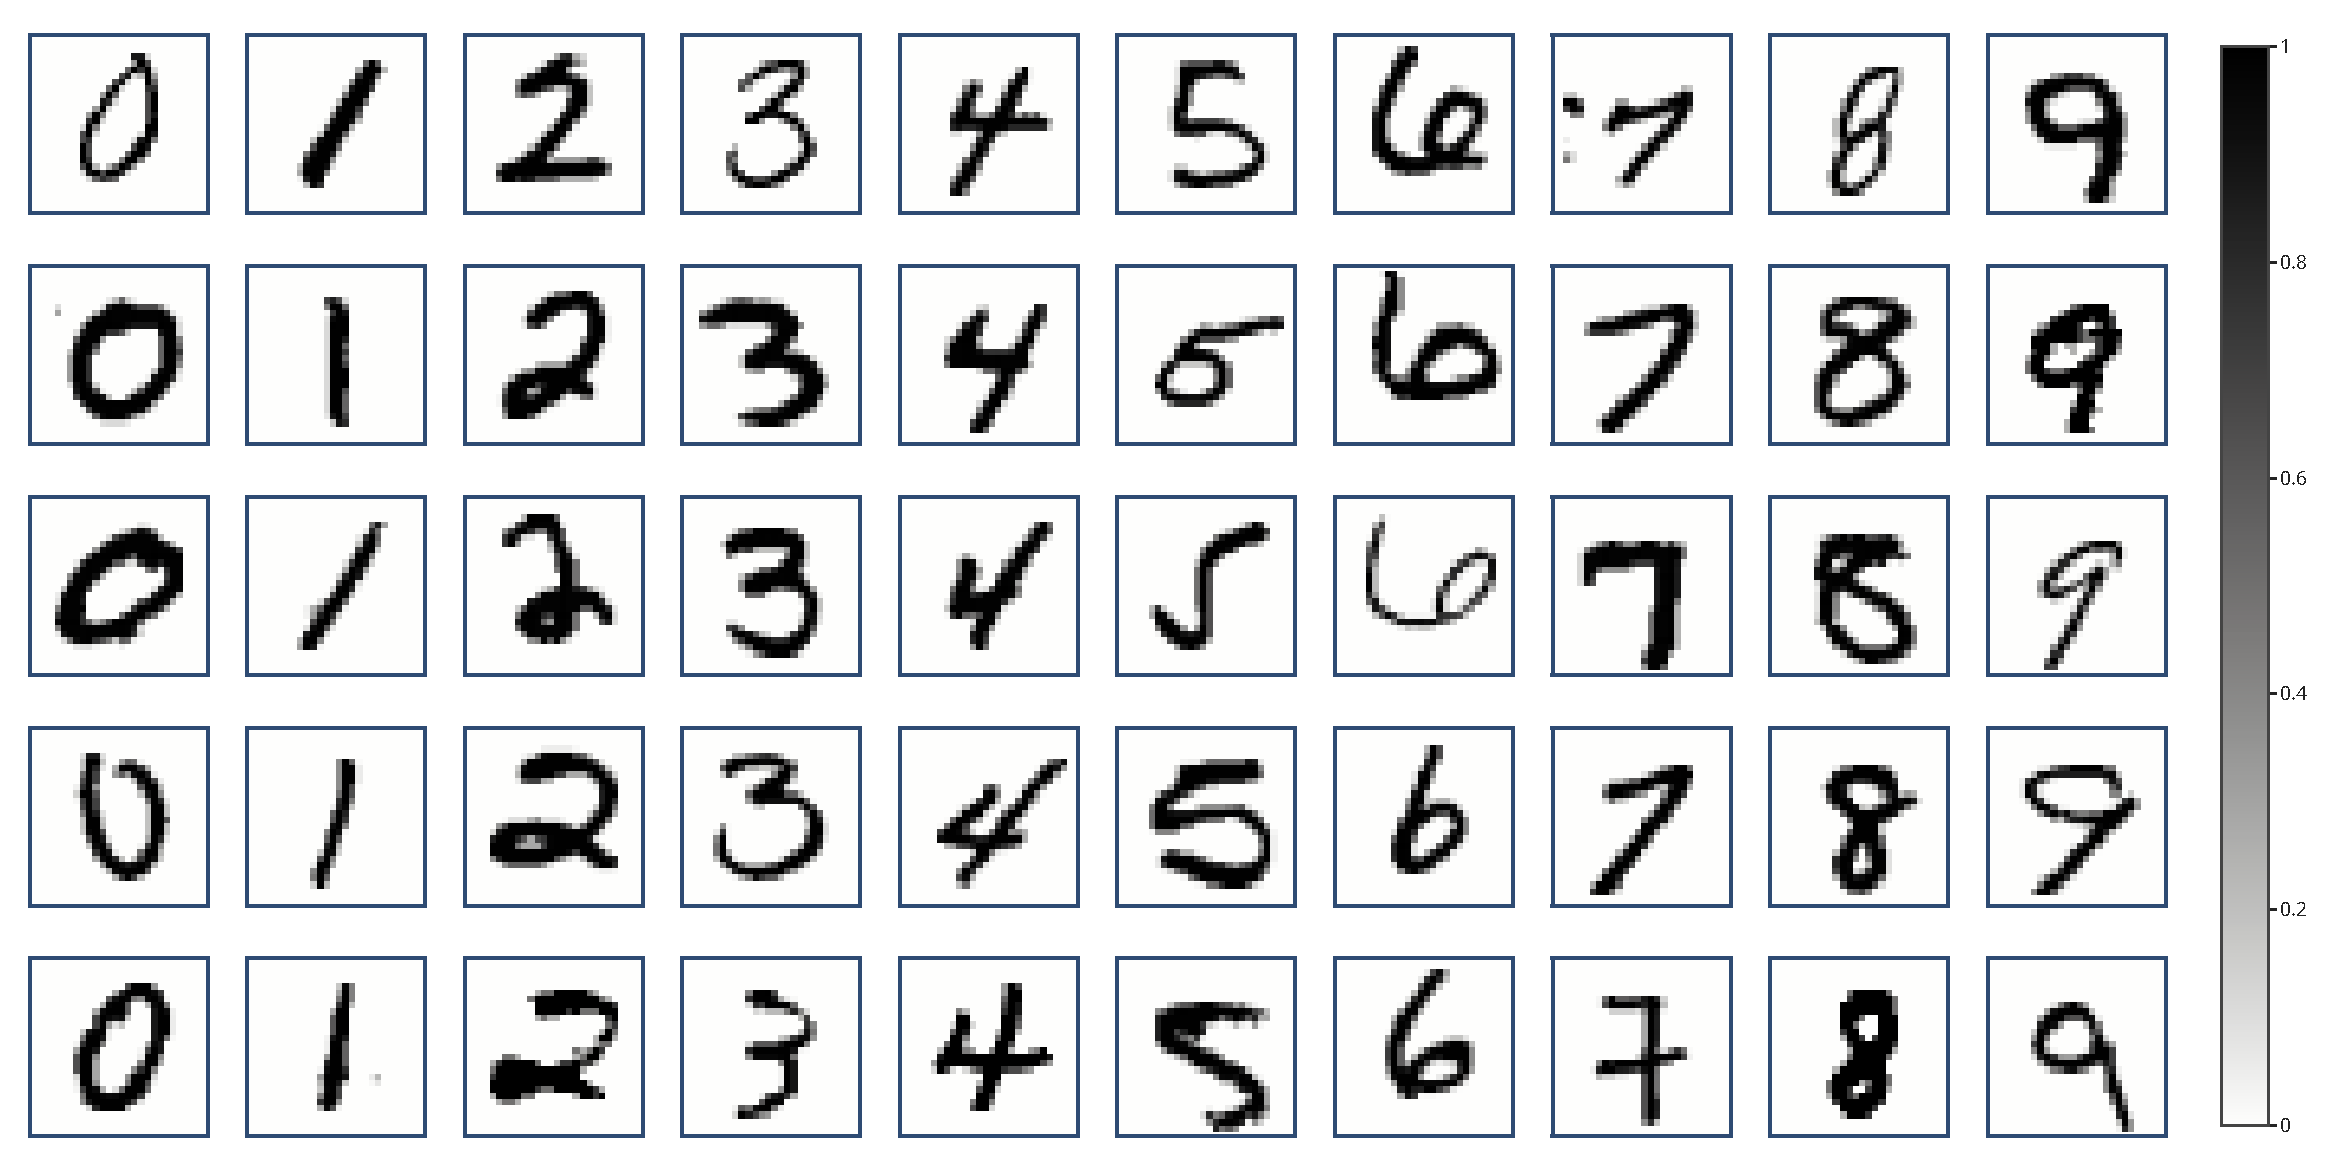
\includegraphics[,
 width=\textwidth,keepaspectratio=true]{MNIST.pdf} 
 
 \caption{Изображения MNIST}
\end{center}
\end{figure}


В этой работе изображения обрезаются так, что используется только центральная область 20$\times$20 пикселей.\\

\subsection{\centering{Особенности архитектуры}}
Нейросетевая архитектура LCSNN \cite{saunders2019locally} вдохновлена строением зрительной коры мозга. $Y$ слой сети состоит из $n$ каналов, каждый из которых является локально соединенным с $X$ слоем нейронов.

\begin{figure}[H] \label{LCSNN}
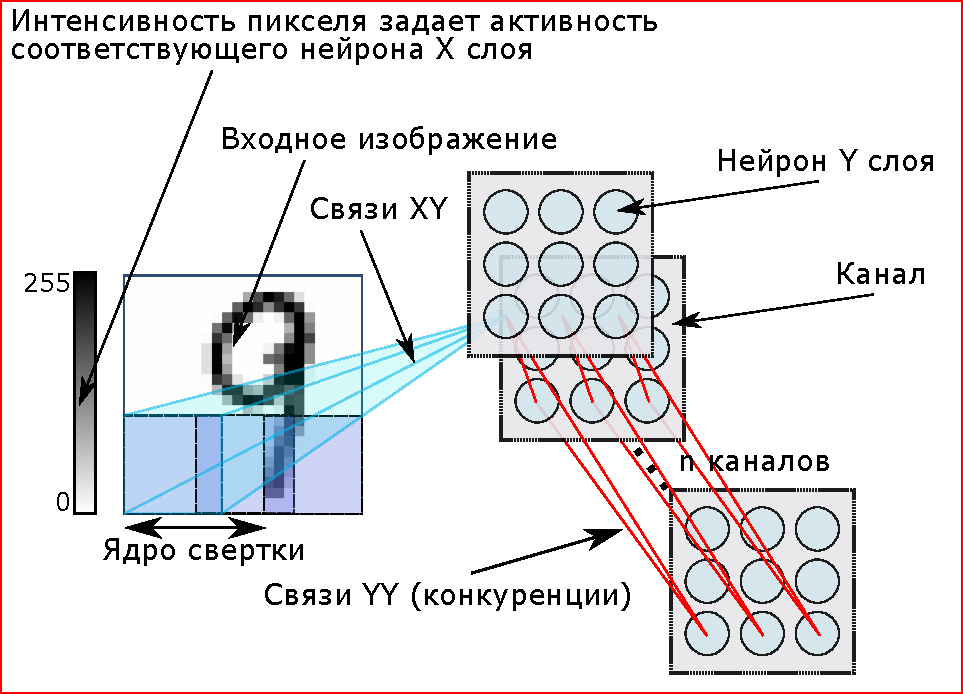
\includegraphics[,
 width=\textwidth,keepaspectratio=true]{LCSNN_ru.pdf} 
    \caption{Схема архитектуры LCSNN} 
\end{figure}

Нейроны, имеющие общие рецептивные поля, соединяются $YY$ связями конкуренции. Такие связи имеют отрицательные веса, а значит, негативно влияют на активность. Нейроны, не имеющие общего рецептивного поля (а значит, реагирующие на разные области изображения) не конкурируют между собой. Связи конкуренции вводятся для улучшения разделения нейронов по выучиваемым признакам.

\subsection{\centering{Обучение связей $XY$}}
Для уменьшения числа параметров модели изображения обрезаются до размера 20$\times$20 пикселей. Края изображений часто практически пусты, поэтому эта операция практически не влияет на объем информации, доступный сети. Для каждого изображения при помощи распределения Пуассона с математическим ожиданием, пропорциональным интенсивности соответствующего пикселя, генерируются $X$ спайки. Обучение связей $XY$ производится по правилу STDP. После каждой итерации обучения производится нормализация весов --- веса каждого нейрона умножаются на такое число, чтобы их сумма стала равной определенной константе. Это делается для избежания возникновения слишком больших отдельных весов. Значение константы нормализации есть важный гиперпараметр модели, который подбирается для каждой конкретной архитектуры.

\begin{figure}[H]
\centering
\begin{subfigure}{0.45\textwidth}
    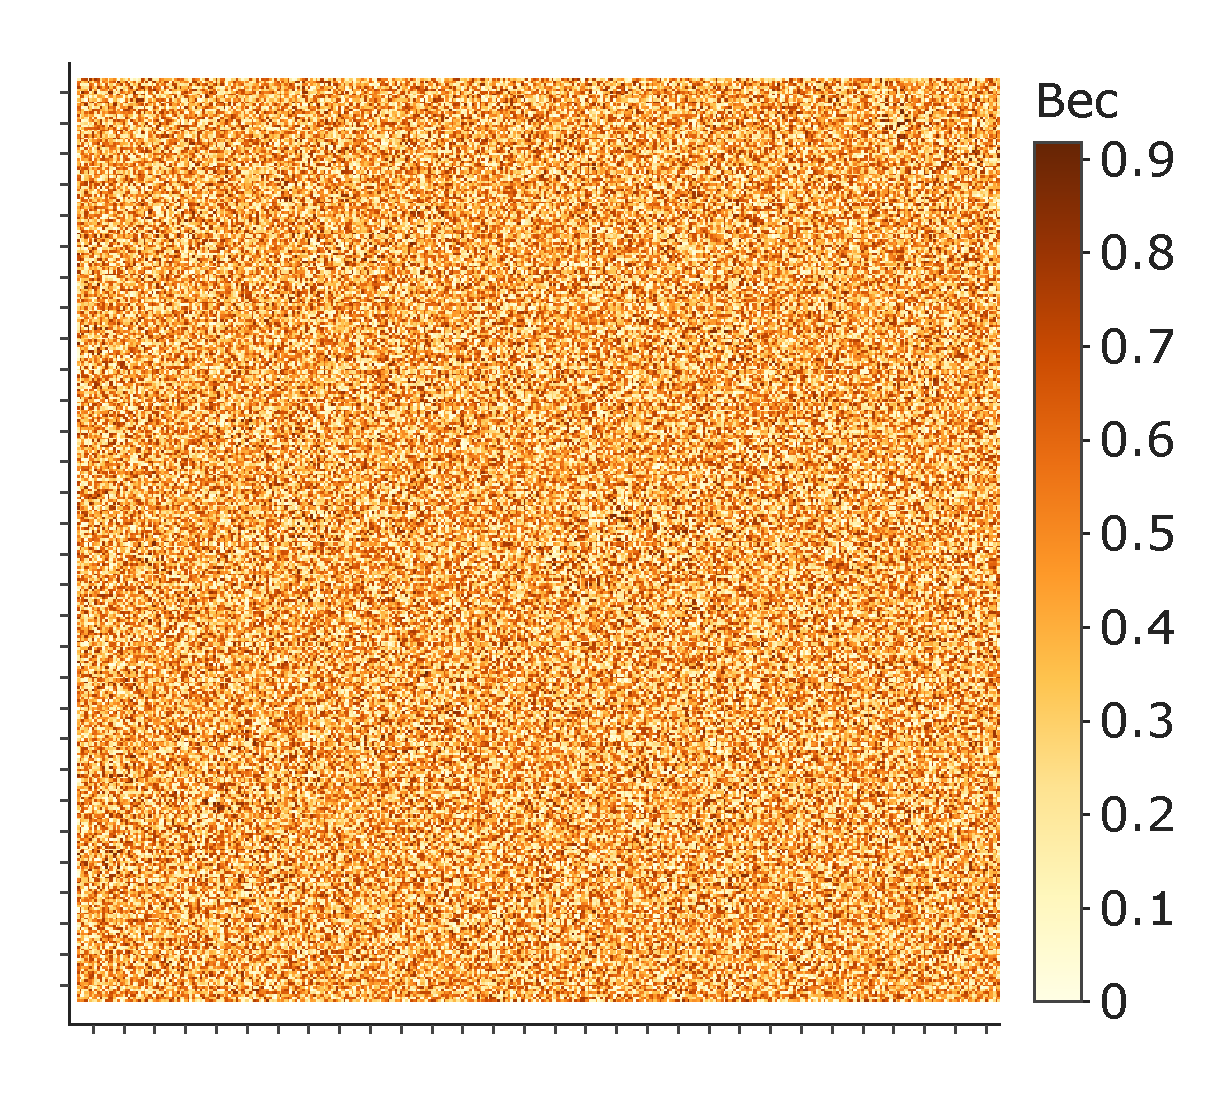
\includegraphics[width=\textwidth,keepaspectratio=true]{weights_XY_untrained_ru.pdf}
    \caption{Веса перед обучением}
\end{subfigure}
\begin{subfigure}{0.45\textwidth}  \label{weights_XY}
    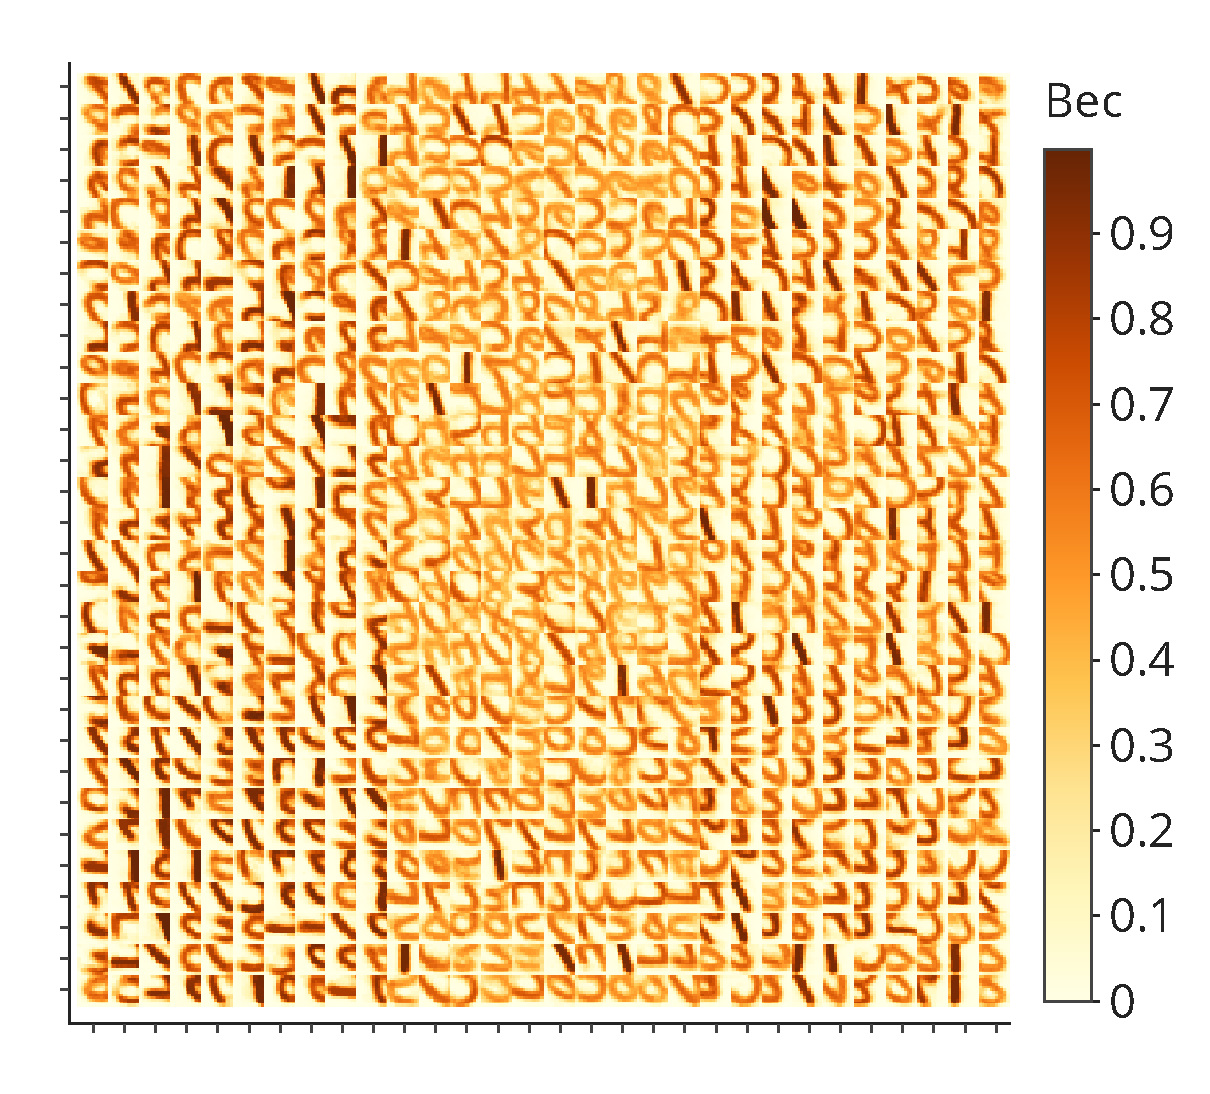
\includegraphics[width=\textwidth,keepaspectratio=true]{weights_XY_ru.pdf}
    \caption{Веса после обучения}
\end{subfigure}
\caption{Визуализация весов $XY$ связей. Каждый квадратик 12$\times$12 соответствует весам одного $Y$ нейрона. Видно, что после обучения нейроны выучивают некоторые признаки, в которых явно угадываются элементы цифр.}
\end{figure}

\subsection{\centering{Интерпретация активности спайковой нейронной сети}}

Для интерпретации активности нейронов $Y$ слоя сети использовалось несколько методов.

\begin{itemize}
 \item Голосование патчей
 \item Общее голосование нейронов
 \item Голосование нейронов с предварительным отбором по спайкам
 \item Линейный классификатор
\end{itemize}

Преимущество первых трех методов заключается в их простоте. Они легко могут быть реализованы на аппаратном уровне. Однако, линейный классификатор значительно превосходит их по точности.\\

\subsubsection{\centering{Калибровка голосов}} \label{calibration}
Для первых трех методов необходимо произвести калибровку голосов нейронов. Каждому нейрону $Y$ слоя ставится в соответствие 10 чисел (голосов) для каждого возможного класса цифр (от 0 до 9). Голос вычисляется как среднее число спайков данного нейрона в ответ на демонстрацию сети данной цифры. Для всех сетей использовалась калибровка на 10000 примерах из калибровочной выборки. Заметим, что калибровка не является частью обучения сети, так как она входит лишь в алгоритм интерпретации поведения сети. Эти голоса используются как мера уверенности нейрона в каждом из классов. После демонстрации изображения сети подсчитывается общее количество спайков для каждого нейрона $Y$ слоя.

\begin{figure}[H]
\centering
\begin{subfigure}{0.9\textwidth}
    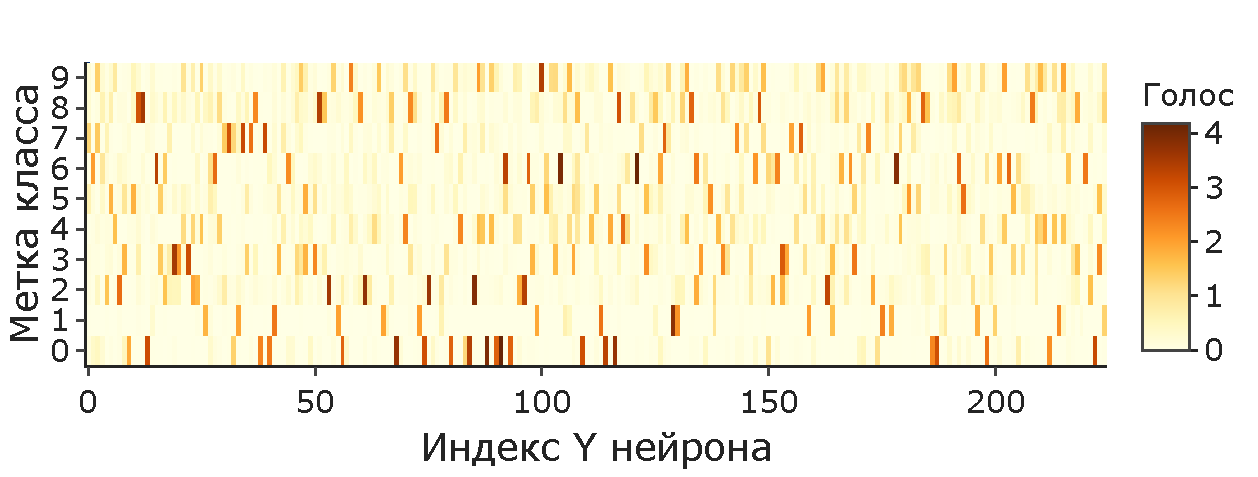
\includegraphics[width=\textwidth,keepaspectratio=true]{votes_ru.pdf}
    \caption{Голоса нейронов.}
\end{subfigure} 
\begin{subfigure}{0.9\textwidth} 
    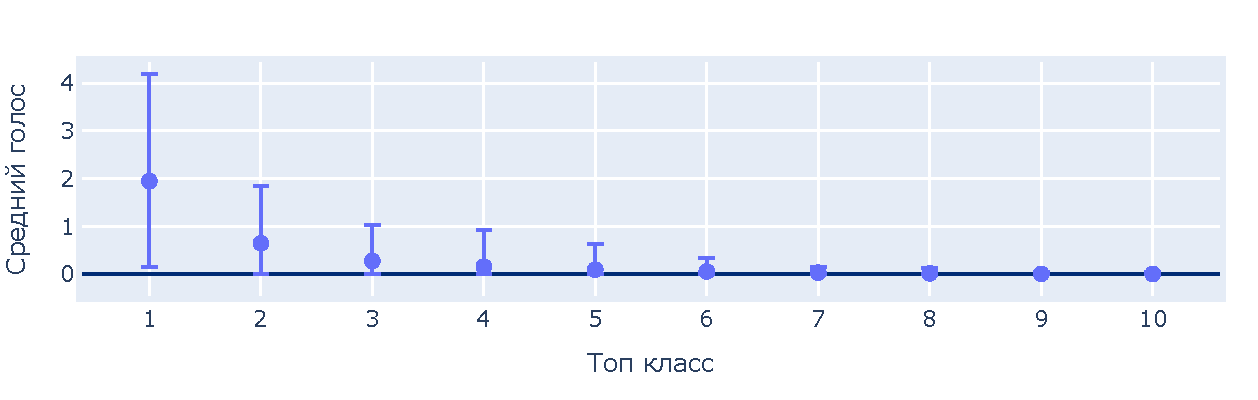
\includegraphics[width=\textwidth,keepaspectratio=true]{votes_distribution_ru.pdf}
    \caption{Среднее значение голоса для топ-n класса, где топ-1 --- класс с максимальным голосом нейрона, топ-10 --- класс с минимальным голосом нейрона.}
\end{subfigure}
\caption{Визуализация голосов нейронов $Y$ слоя. Высокие значения соответствуют большой специализации нейрона на соответствующем классе.}
\end{figure}

 Далее результатом будем называть произведение количества спайков нейрона на голос.

\begin{center}
 Общее голосование
\end{center}
Ответом сети считается класс с максимальным результатом среди всех нейронов.

\begin{center}
 Голосование патчей
\end{center}
Для каждого рецептивного поля ищется нейрон с максимальным результатом. Ответом сети считается класс с максимальным результатом среди этих нейронов. 

\begin{center}
 Отбор по спайкам
\end{center}
Для каждого рецептивного поля ищется нейрон с максимальным количеством спайков. Ответом сети считается класс с максимальным результатом среди этих нейронов.

\begin{center}
 Линейный классификатор
\end{center}
Суммы спайков нейронов $Y$ слоя используются для обучения линейного классификатора. Для обучения классификатора также используется калибровочная выборка.

\begin{center}
 Оценка алгоритма интерпретации активности
\end{center}
Для оценки работы алгоритма интерпретации используется точность --- отношение количества верно распознанных цифр к размеру тестовой выборки. В этой работе во всех случаях размер тестовой выборки составляет 10000. 

\subsubsection{\centering{Сравнение алгоритмов интерпретации активности сети}}
LCSNN отличаются большой скоростью обучения. Были построены кривые обучения для различных алгоритмов интерпретации активности сети. Точность измерялась через каждые 250 итераций обучения. Для калибровки алгоритма интерпретации использовалась калибровочная выборка объемом 5000. Для измерения точности использовалась тестовая выборка объемом 1000.

Видно, что через несколько тысяч итераций обучения точность распознавания выходит на плато насыщения, после чего уже не возрастает. Видно, что три метода голосования в целом не отличаются по точности, а линейный классификатор значительно превосходит их все. Заметим, что точность даже необученной сети может достигать 70\% за счет калибровки механизма интерпретации.

\begin{center}
\begin{figure}[H] 
 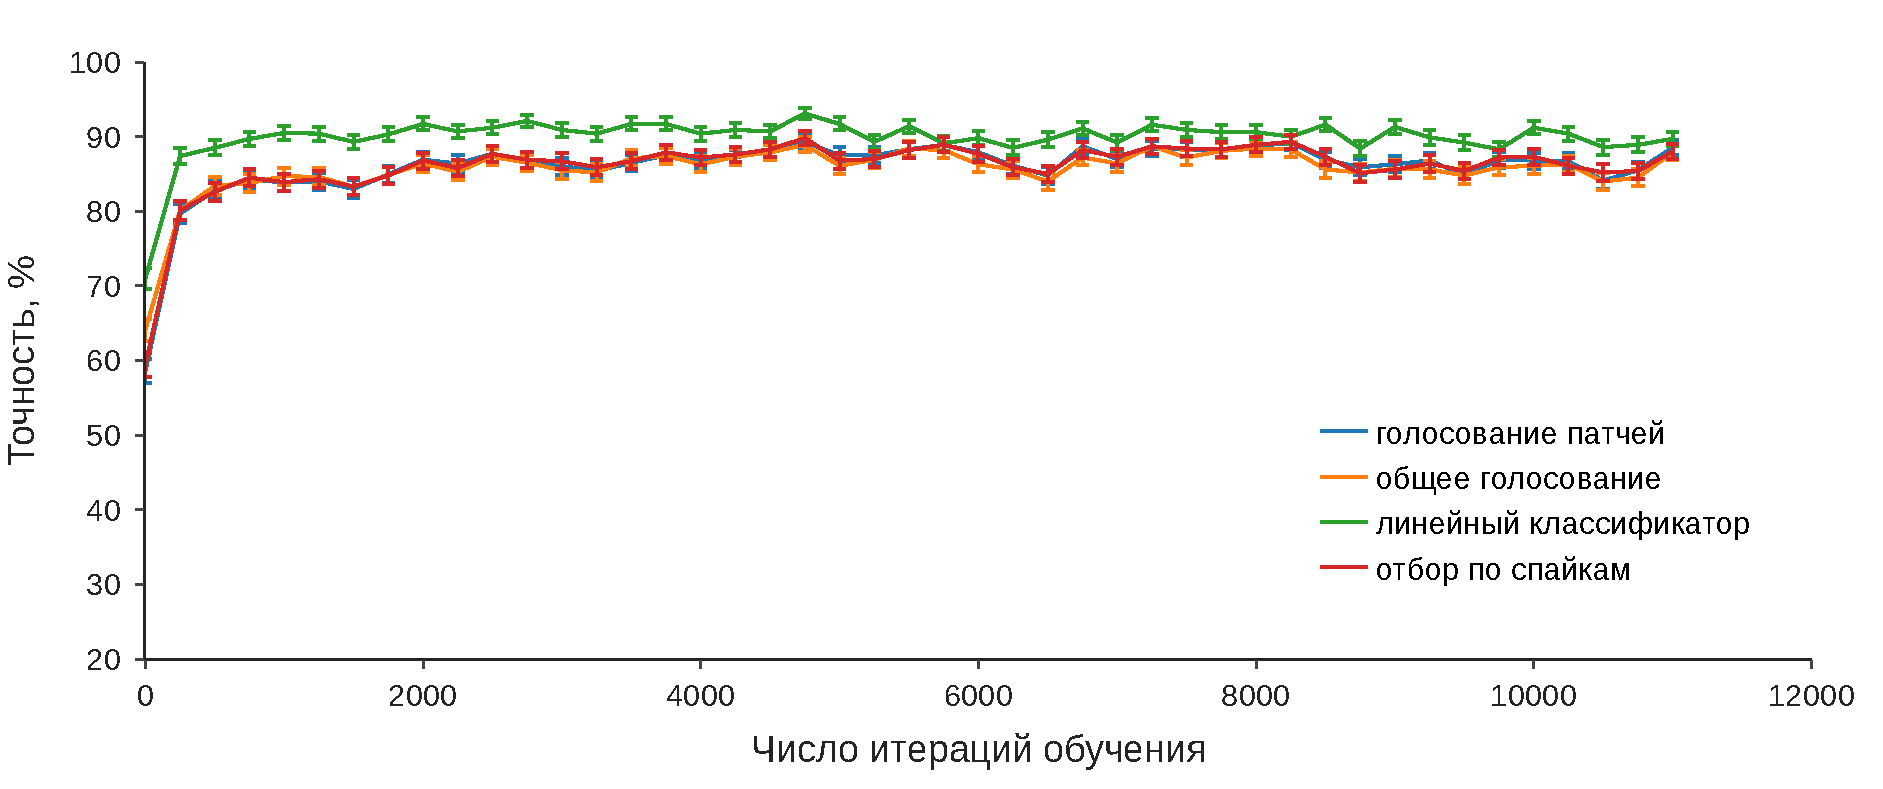
\includegraphics[width=\textwidth,keepaspectratio=true]{LCSNN_learning_rate_ru.pdf}
 \caption{Скорость обучения LCSNN. Сравнение различных алгоритмов интерпретации активности.}
\end{figure}
\end{center}


\subsection{\centering{Сравнение эффективности операции свертки и локального рецептивного поля}}
Были проведены эксперименты по измерению точности сетей с различными архитектурами. Для сверточных и полносвязных сетей вводились аналогичные связи конкуренции. Из-за очень высоких вычислительных нагрузок не ставилось задачи по нахождению параметров, идеально обеспечивающих максимальную точность для каждой архитектуры. Эти параметры были подобраны приблизительно, поэтому могли не попасть в максимум точности, однако величина расхождения не превышает 1-2\%. Все точности посчитаны при помощи алгоритма интерпретации активности на основе голосования нейронов (учитывался лучший результат). Заметим, что при использовании линейного классификатора в качестве алгоритма интерпретации удалось достигнуть 95\% точности для локально соединенной сети из 1000 каналов с размером ядра 12.

\begin{table}[H]
 \caption{Результаты сравнения различных архитектур спайковых нейронных сетей. Для каждой сети точность измерялась $N=5$ раз. В таблице указаны средние значения и стандартное отклонение для точности.}
\begin{center}
\begin{tabular}{|l|l|l|l|l|l|l|}
\hline
Архитектура & Каналы & Ядро & Веса & Нейроны & Точность, \% \\
\hline
{LCSNN} & {100} & {12} & {449100} & {900} & {$87.5 \pm 0.9$}\\
\hline
{LCSNN} & {100} & {8} & {798400} & {1600} & {$82.9 \pm 0.2$}\\
\hline
{LCSNN\footnotemark} & {25} & {12} & {95400} & {225} & {$82.3 \pm 1.0$}\\
\hline
{LCSNN} & {25} & {12} & {95400} & {225} & {$80.1 \pm 1.0$}\\
\hline
{LCSNN} & {25} & {8} & {169600} & {400} & {$73.6 \pm 1.0$}\\
\hline
{CSNN} & {81} & {12} & {543105} & {729} & {$77.2 \pm 1.7$}\\
\hline
{CSNN} & {100} & {8} & {11350} & {1600} & {$77.4 \pm 1.9$}\\
\hline
{CSNN} & {25} & {12} & {3900} & {225} & {$65.8 \pm 0.7$}\\
\hline
{CSNN} & {25} & {8} & {1900} & {400} & {$63.1 \pm 1.2$}\\
\hline
{FCSNN} & {100} & {20} & {44950} & {100} & {$73.4 \pm 0.9$}\\
\hline
\end{tabular}
\end{center}
\end{table}

\footnotetext{Сеть с обучением связей конкуренции}

Видно, что локально соединенная сеть превосходит сверточную сеть по точности даже при чуть превышающем числе параметров последней. Также видно, что не следует использовать слишком маленький размер ядра свертки. Это приводит к выучиванию сетью менее значительных признаков. В классическом машинном обучении используются либо неглубокие сети с большими ядрами свертки, либо глубокие сети с маленькими ядрами свертки.

Заметим, что спайковые нейронные сети могут достигать значительно больших точностей на MNIST. Для этого можно использовать:
\begin{itemize}
\item Сети с существенно большим числом параметров, чем в этой работе
\item Более глубокие сети с большим количеством слоев
\item Другие алгоритмы обучения (например, обучение с учителем)
\end{itemize}

\begin{table}[H]
 \caption{Результаты других исследований спайковых нейронных сетей. Во всех используется датасет MNIST.}
\begin{center}
\begin{tabular}{|l|p{4cm}|p{7cm}|l|l|}
\hline
Статья & Архитектура & Обучение & Точность, \% \\
\hline
{\cite{saunders2019locally}} & {Локальная + конкуренция} & {Без учителя} & {$95.07 \pm 0.63$}\\
\hline
{\cite{mnist1}} & {Полносвязная + конкуренция} & {Без учителя} & {95}\\
\hline
{\cite{MaxActiv1}} & {Полносвязная + конкуренция} & {С учителем / с частичным привлечением учителя} & {95.4 / 72.1}\\
\hline
{\cite{conv1}} & {Сверточная} & {С частичным привлечением учителя} & {$96.95 \pm 0.08$}\\
\hline
{\cite{conv2}} & {Сверточная} & {С частичным привлечением учителя} & {$99.28 \pm 0.1$}\\
\hline
{\cite{conv3}} & {Сверточная} & {С частичным привлечением учителя} & {$97.20 \pm 0.07$}\\
\hline
\end{tabular}
\end{center}
\end{table}

Результат, полученный в этой работе, практически соответствует результату из первой строки.

\subsection{\centering{Обучение связей $YY$ (конкуренции)}}
Связи $YY$ очень сильно влияют на обучение связей $XY$. Большие по модулю значения способствуют вариативности в обучении $Y$ нейронов, так для каждого рецептивного поля одновременно активными не могут быть нейроны, имеющие схожие веса $XY$. Малые по модулю значения не позволяют нейронам специализироваться. 

Примечательно, что с такими большими по модулю значениями весов конкуренции для каждого рецептивного поля остается активным лишь один нейрон (или иногда несколько нейронов), веса которого лучше всего соответствует области представленного изображения, который подавляет активность остальных.

\begin{figure}[H]
\centering
\begin{subfigure}{0.95\textwidth}
    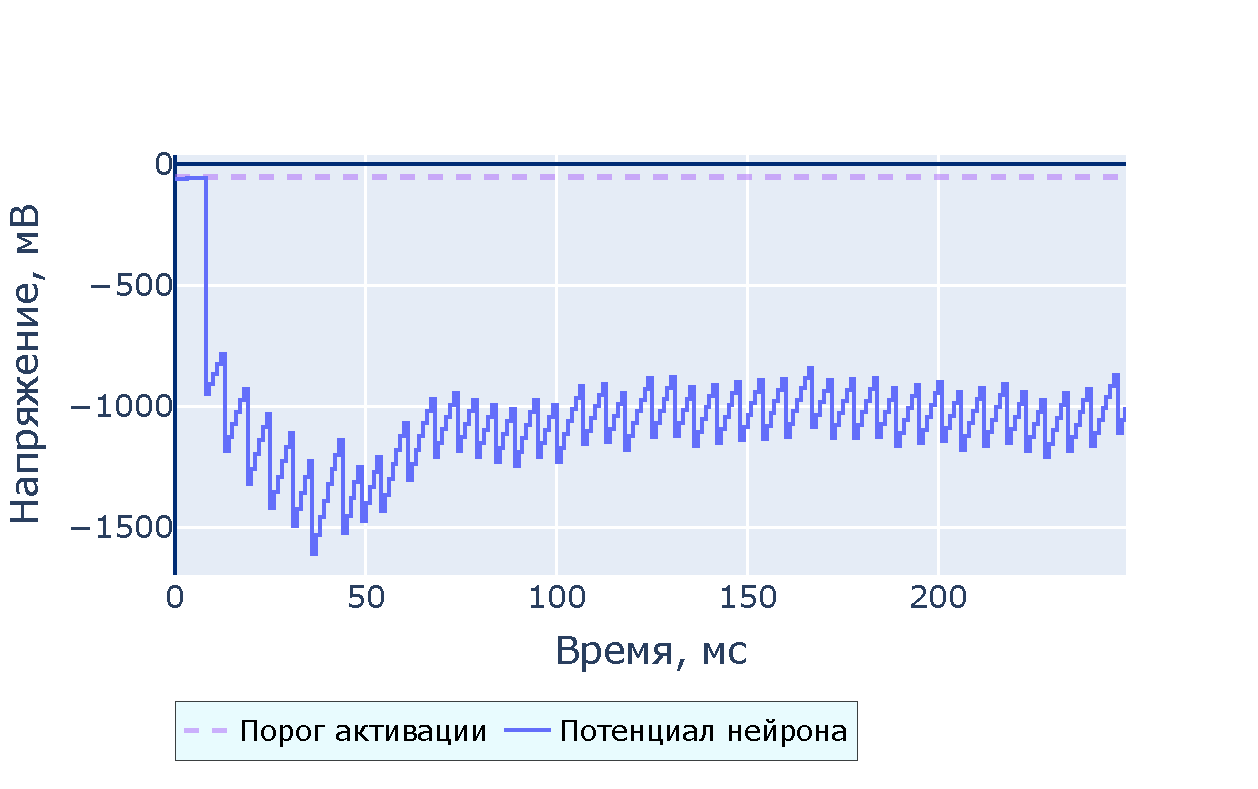
\includegraphics[width=\textwidth,keepaspectratio=true]{bad_voltage_ru.pdf}
    \caption{Активность нейрона, который проиграл в конкуренции, подавлена другими нейронами.
    } 
\end{subfigure}
\begin{subfigure}{0.95\textwidth}
    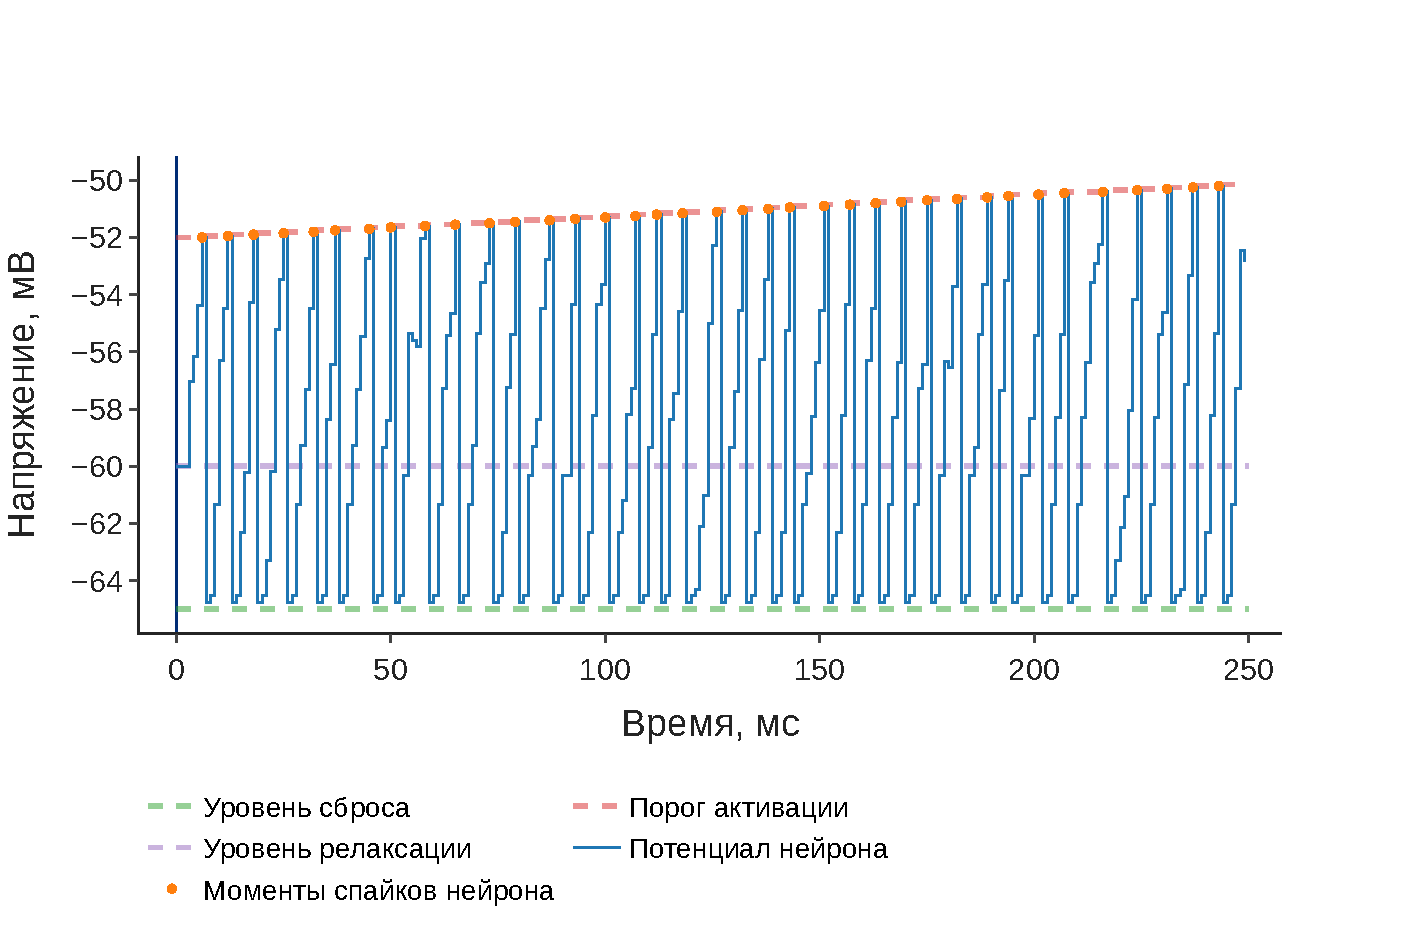
\includegraphics[width=\textwidth,keepaspectratio=true]{good_voltage_ru.pdf}
    \caption{Активность нейрона, который выиграл в конкуренции. Присутствуют множество спайков.}
\end{subfigure}
\caption{Влияние конкуренции на активность нейронов\\
\textit{Примечание: на графике слева не представлены значения $v_{rest}$ и $v_{reset}$, так как на данном масштабе они практически совпадают с $v_{thresh}$.}}
\label{competition-training-importance}  
\end{figure} 

\begin{figure}[H]
\centering
\begin{subfigure}{0.45\textwidth}
    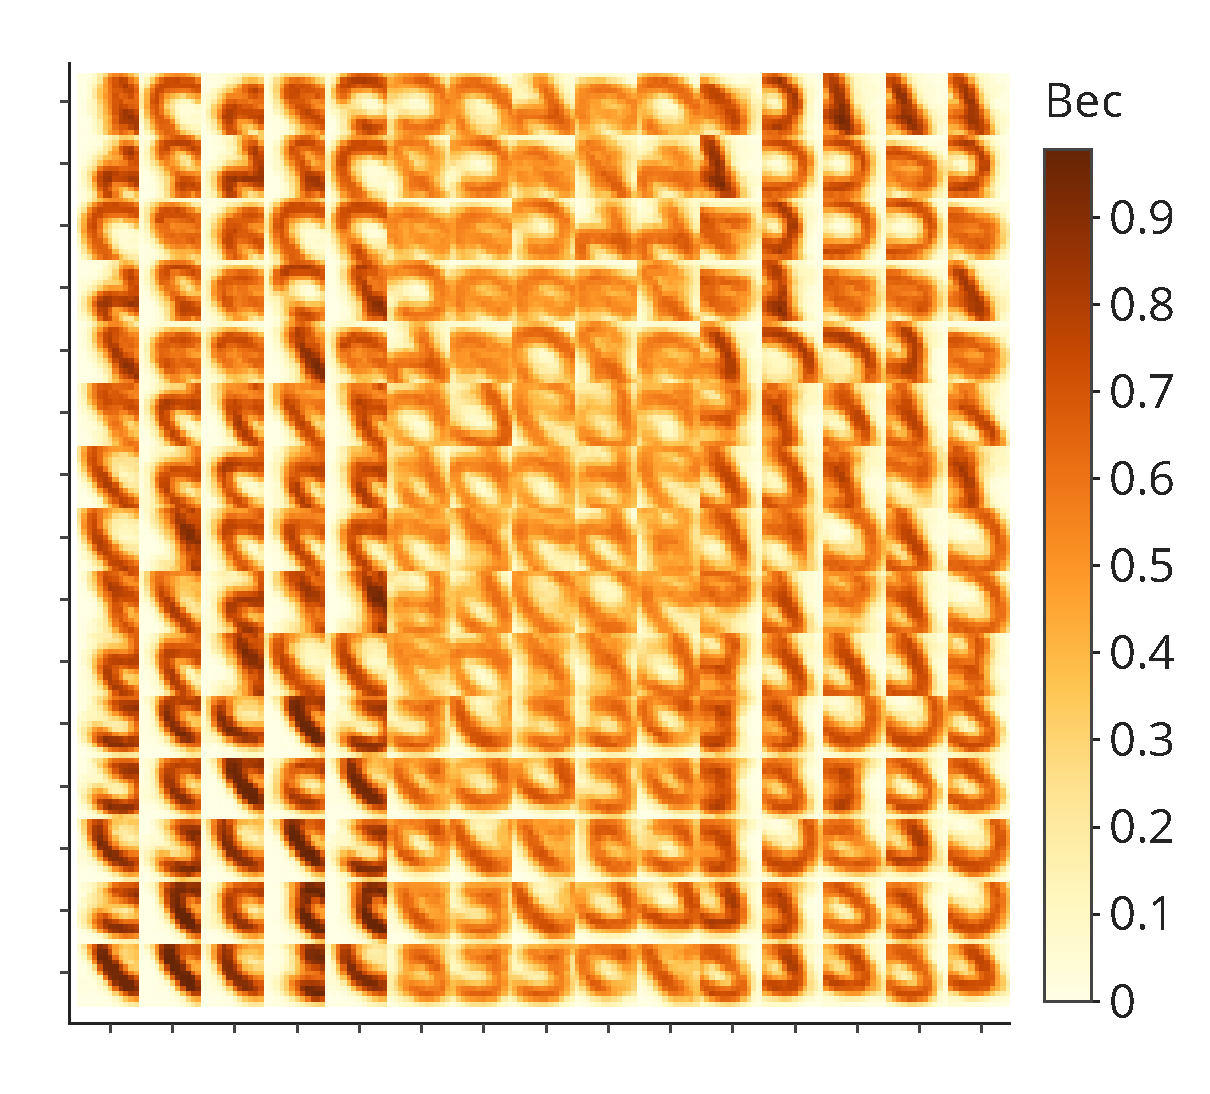
\includegraphics[width=\textwidth,keepaspectratio=true]{weights_XY_bad_ru.pdf}
    \caption{Слабо специализированные веса,\\ вес конкуренции равен --10.}
\end{subfigure}
\begin{subfigure}{0.45\textwidth}
    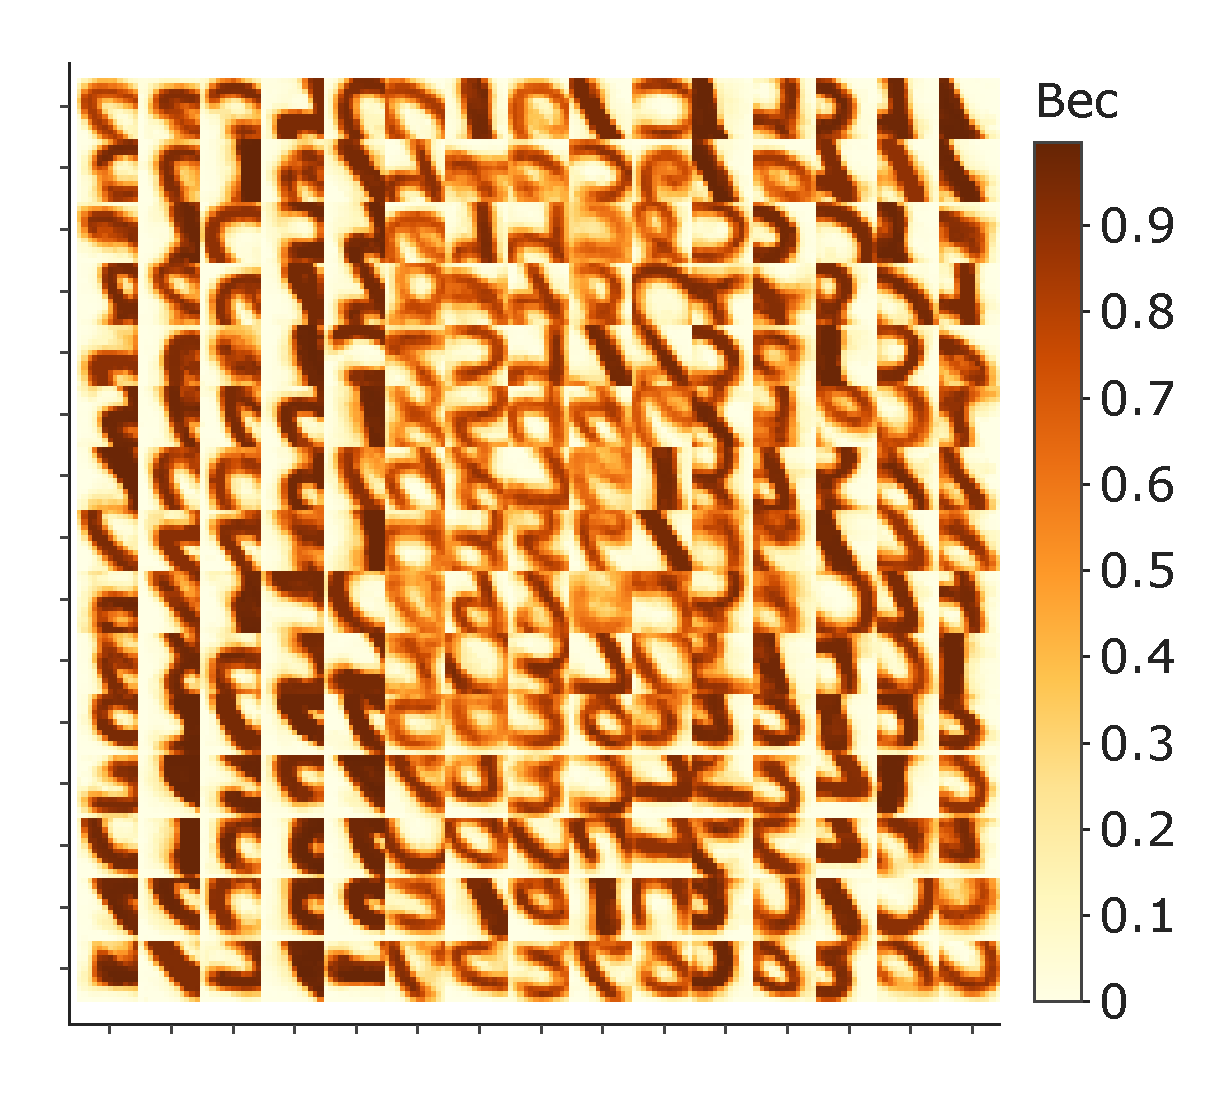
\includegraphics[width=\textwidth,keepaspectratio=true]{weights_XY_good_ru.pdf}
    \caption{Специализированные веса,\\ вес конкуренции равен --100.}
\end{subfigure}
\caption{Влияние конкуренции на обучение связей $XY$.}
\label{competition-training-importance}
\end{figure}

Все сети до этого момента имели фиксированные веса конкуренции. Было обнаружено, что обучение весов конкуренции позволяет повысить точность сети. Для обучения связей $YY$ используется правило anti-STP (\autoref{sec:anti-STDP}). При помощи варьирования параметров этого правила были получены различные распределения весов конкуренции.

\begin{figure}[H]
\centering
\begin{subfigure}{0.45\textwidth}
    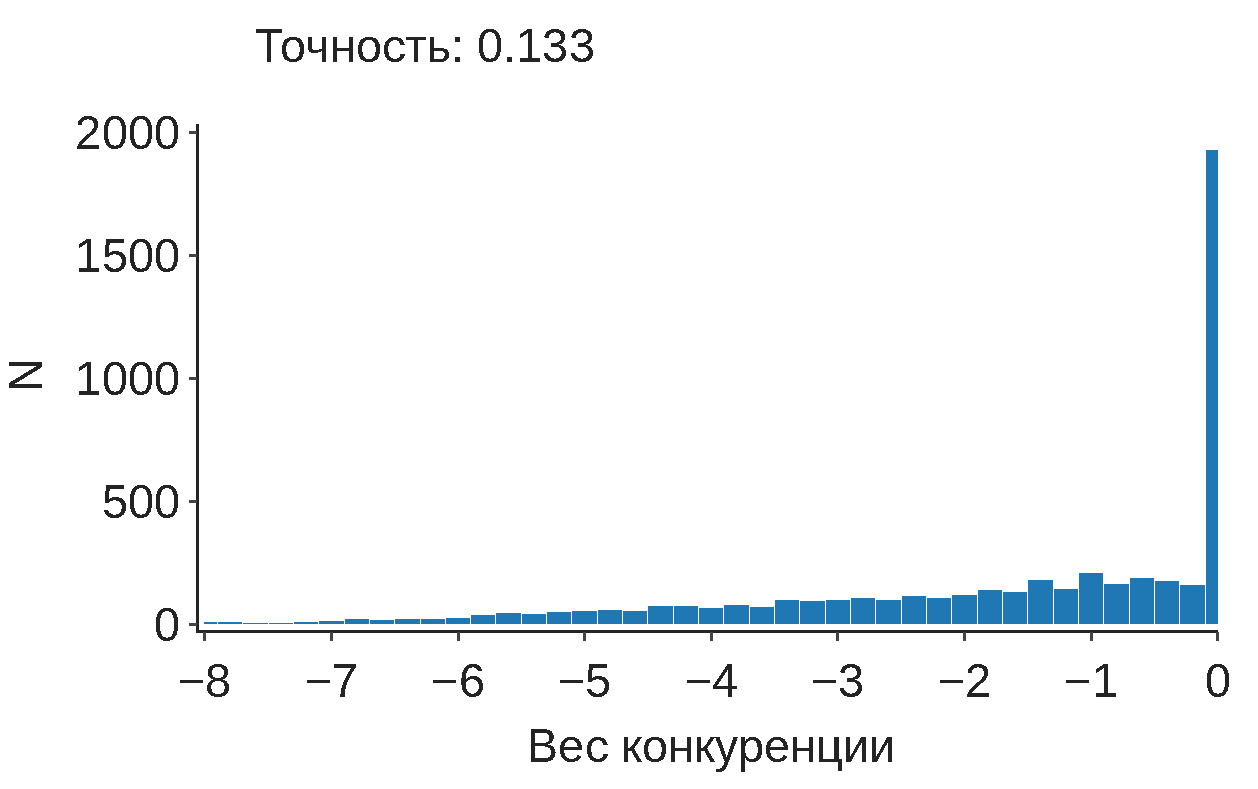
\includegraphics[width=\textwidth,keepaspectratio=true]{competition_distribution_worst_ru.pdf}
    \caption{Очень слабая конкуренция}
\end{subfigure}
\begin{subfigure}{0.45\textwidth}
    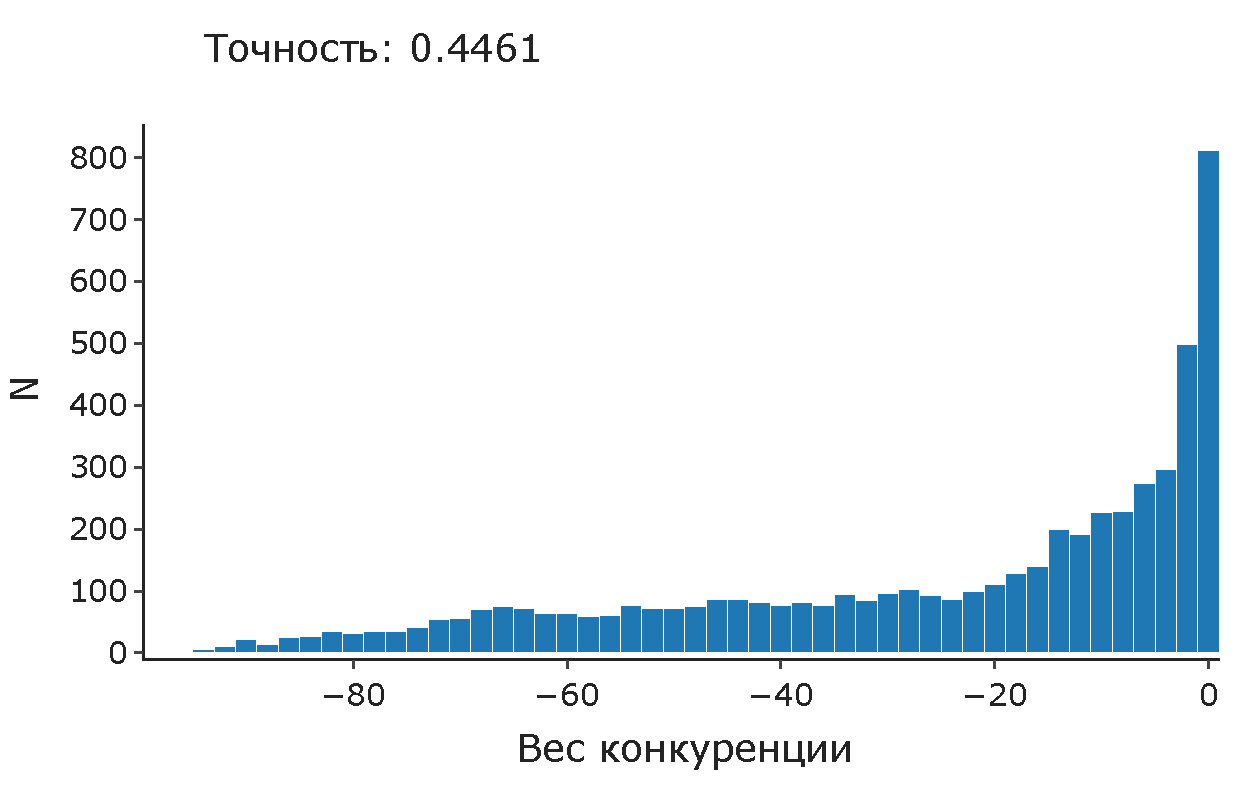
\includegraphics[width=\textwidth,keepaspectratio=true]{competition_distribution_medium_bad_ru.pdf}
    \caption{Слабая конкуренция}
\end{subfigure}
\\
\begin{subfigure}{0.45\textwidth}
    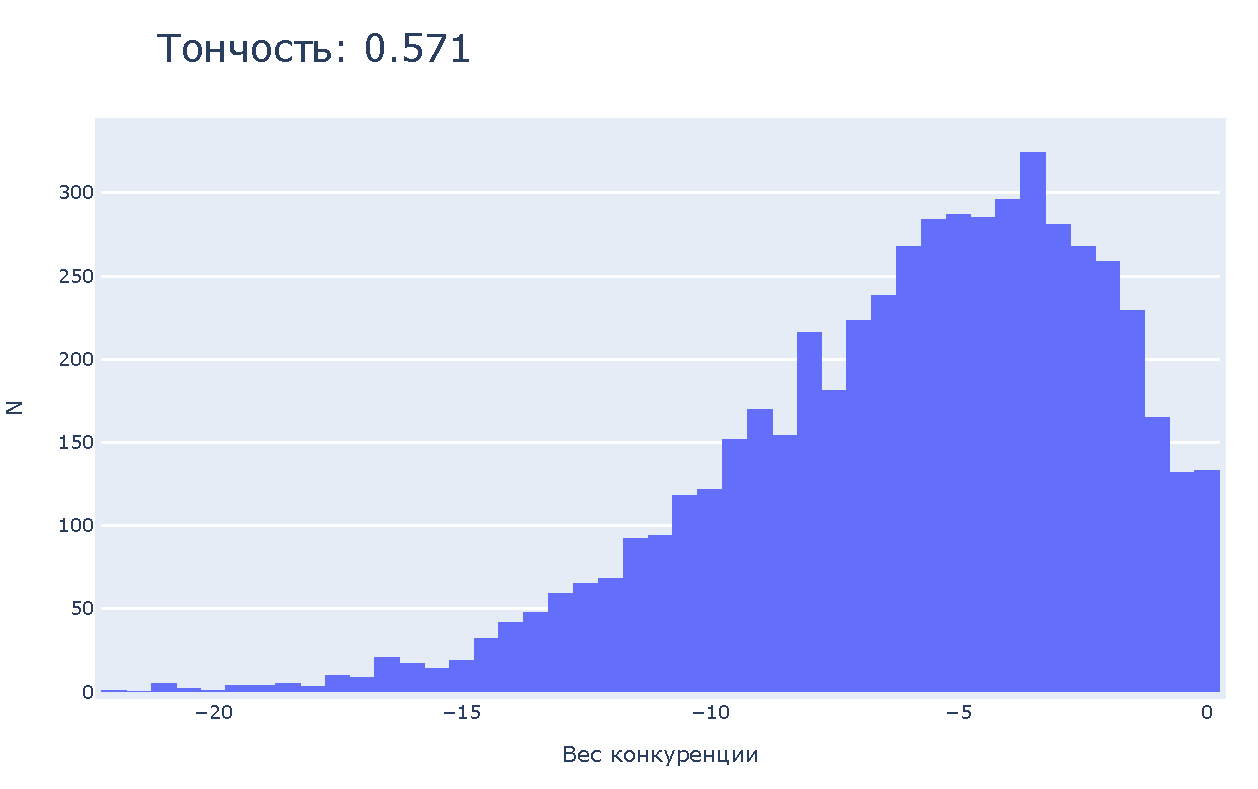
\includegraphics[width=\textwidth,keepaspectratio=true]{competition_distribution_medium_good_ru.pdf}
    \caption{Средняя конкуренция} 
\end{subfigure}
\begin{subfigure}{0.45\textwidth}
    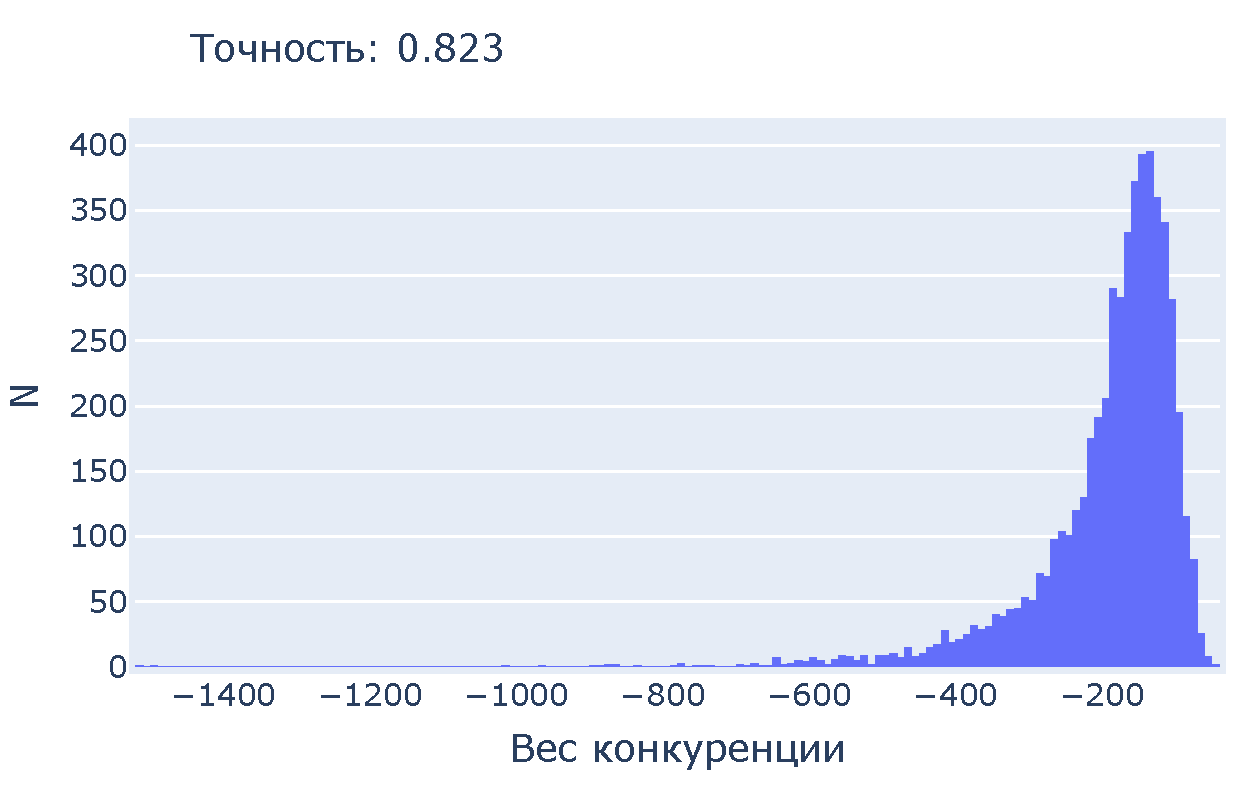
\includegraphics[width=\textwidth,keepaspectratio=true]{competition_distribution_best_ru.pdf}
    \caption{Сильная конкуренция}
\end{subfigure}
\caption{Различные распределения весов конкуренции}
\label{fig:competition_distributions}
\end{figure}

Видно, что точность сети повышается при тяготении распределения весов конкуренции в сторону больших по модулю значений. Заметим, что целью являлось не нахождение параметров сети, обеспечивающих максимальную точность, а исследования влияния обучения или не-обучения конкуренции на точность сети с данной конфигурацией остальных параметров.

Примечательно, что не все связи $YY$ получают большие по модулю значения. Это объясняется тем, что нейроны, специализирующиеся на значительно разных признаках, не нуждаются в конкуренции, так как они не проявляют высокую активность одновременно.

\begin{figure}[H]
\centering
\begin{subfigure}{0.45\textwidth}
    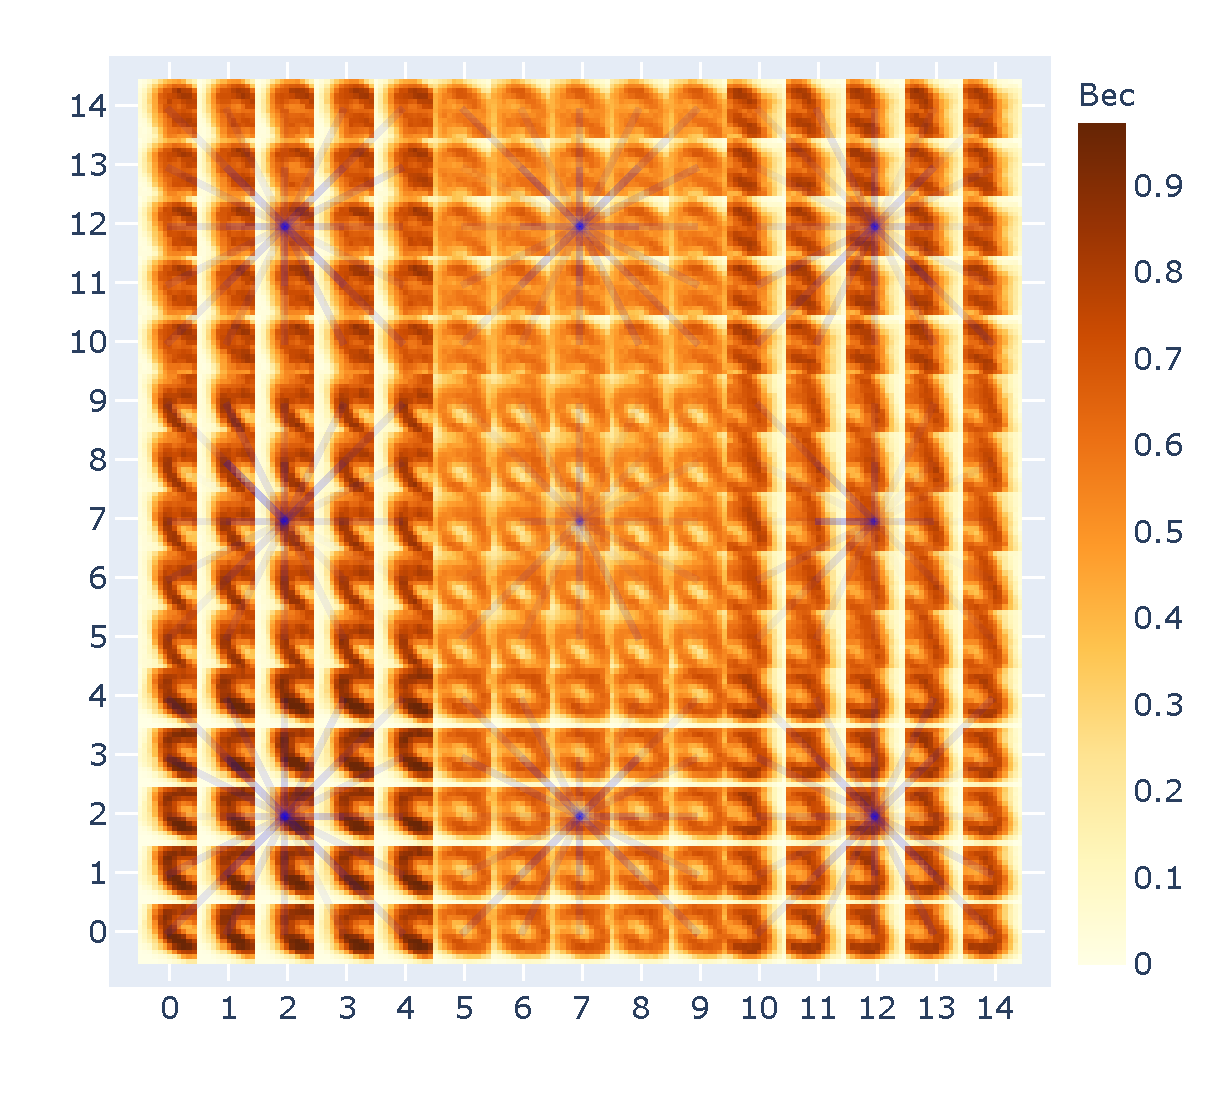
\includegraphics[width=\textwidth,keepaspectratio=true]{competition_on_XY_worst_ru.pdf}
    \caption{Очень слабая конкуренция}
\end{subfigure}
\begin{subfigure}{0.45\textwidth}
    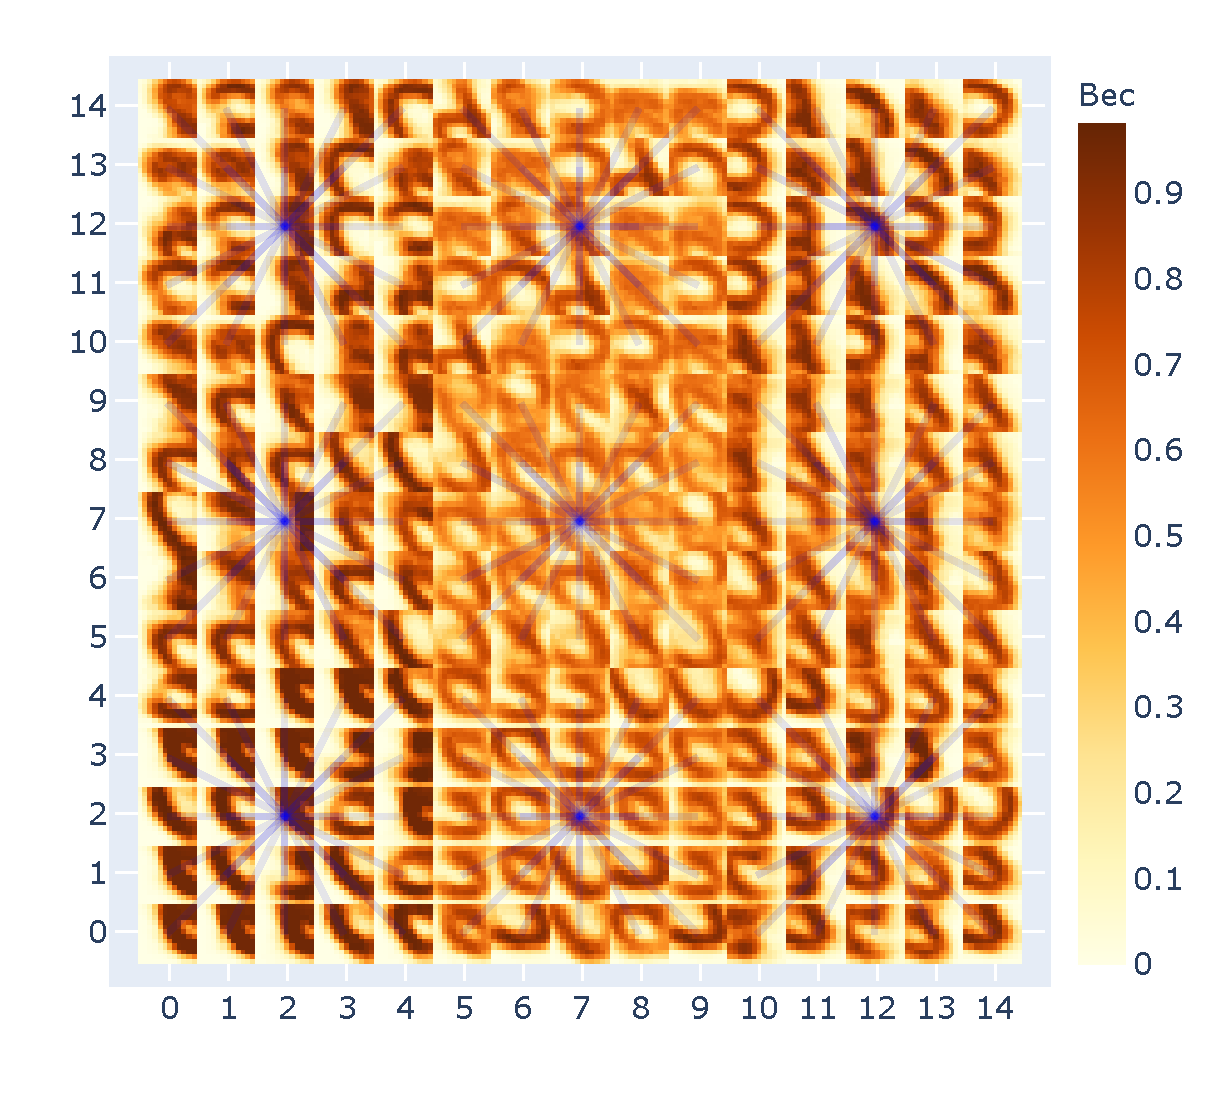
\includegraphics[width=\textwidth,keepaspectratio=true]{competition_on_XY_medium_bad_ru.pdf}
    \caption{Слабая конкуренция}
\end{subfigure}
\\
\begin{subfigure}{0.45\textwidth}
    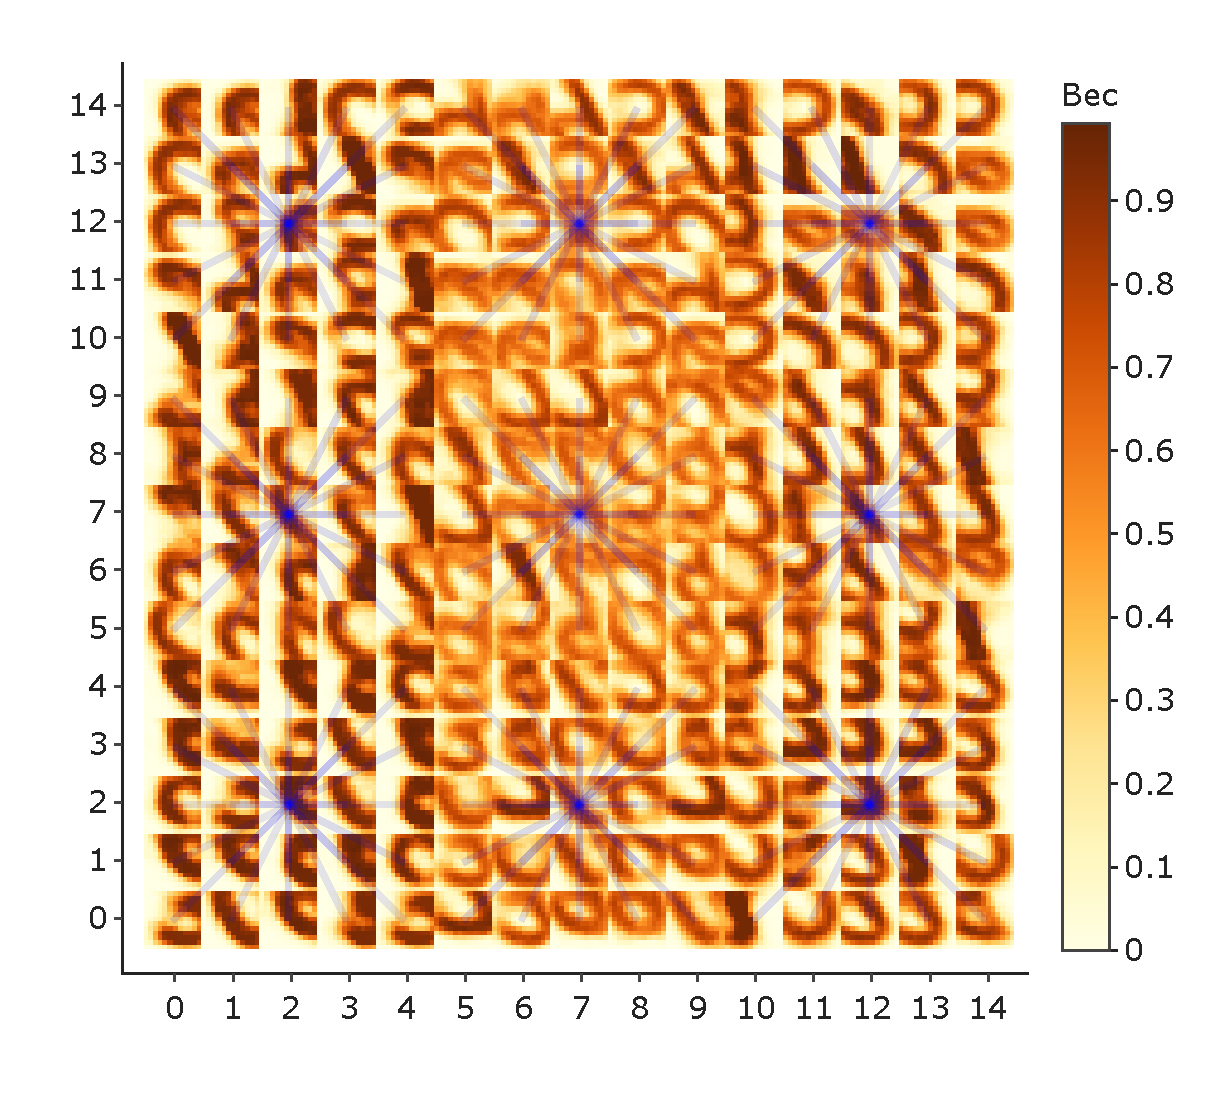
\includegraphics[width=\textwidth,keepaspectratio=true]{competition_on_XY_medium_good_ru.pdf}
    \caption{Средняя конкуренция} 
\end{subfigure}
\begin{subfigure}{0.45\textwidth}
    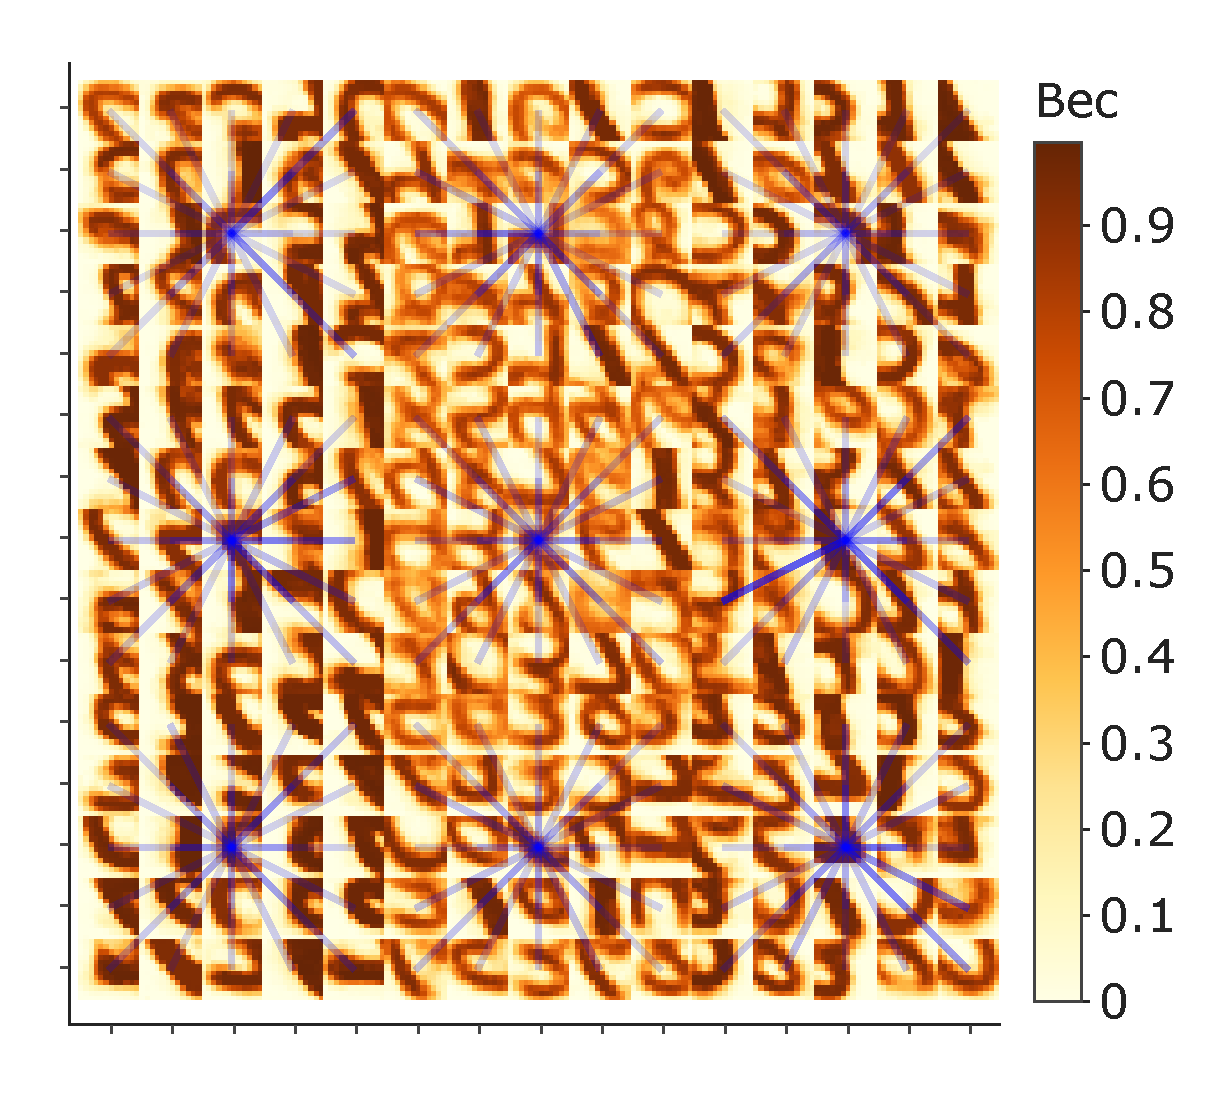
\includegraphics[width=\textwidth,keepaspectratio=true]{competition_on_XY_best_ru.pdf}
    \caption{Сильная конкуренция}
\end{subfigure} 
\caption{Визуализация весов конкуренции поверх весов $XY$. Изображения соответствуют весам сетей с рисунка \ref{fig:competition_distributions}. Изображены только веса конкуренции для одного нейрона в каждом рецептивном поле для избегания загромождения визуализации. Насыщенный синий цвет соответствует большей по модулю конкуренции (используется среднее арифметическое между весов $W_{ij}$ и $W_{ji}$). Видно, что похожие признаки сильнее конкурируют между собой, чем различные.}
\end{figure}

\addcontentsline{toc}{subsection}{Выводы к разделу 3}
\subsection*{\centering{Выводы к разделу 3}} 
В результате сравнения архитектур было показано, что локально соединенная архитектура превосходит
сверточную архитектуру по точности при сравнимом числе параметров. Также было показано, что обучение связей конкуренции способно улучшить точность спайковой сети. Полученные результаты соответствуют state of the art.

\pagebreak

\addcontentsline{toc}{section}{Выводы}
\section*{\centering{Выводы}}
В результата проведения работы было проведено сравнение локально соединенной спайковой нейронной сети со сверточной спайковой нейронной сетью. Оказалось, что локально соединенная архитектура значительно превосходит сверточную по точности при примерно одинаковом числе параметров.

Также было обнаружено, что обучение конкуренции позволяет дополнительно повысить точность сети.

\addcontentsline{toc}{section}{Заключение}
\section*{\centering{Заключение}}
Локально соединенная сеть – перспективная нейросетевая архитектура, подходящая для реализации на вычислительном нейрочипе. Способность быстро выходить на плато кривой обучения позволяет использовать локально соединенные сети для обучения на выборках сравнительно небольшого объема (3000-5000). Использование дополнительного алгоритма интерпретации активности, такого как линейный классификатор, позволяет повысить эффективность сети.

Число параметров (весов) сети определяет энергоэффективность мемристорного нейрочипа, так как каждый вес обычно представлен физическим элементом. Таким образом, это главный фактор, определяющий эффективность любой модели. Было показано, что локально соединенная сеть превосходит сверточную в точности при примерно одинаковом числе параметров.

Также было показано, что при помощи обучения связей конкуренции можно добиться большей точности, чем при фиксированных весах конкуренции.

В качестве перспектив для дальнейшего исследования можно отметить более глубокое изучение обучения конкуренции, а именно анализ распределений весов конкуренции, а также подбор оптимальных параметров обучения конкуренции. В этой работе не было исследовано обучение конкуренции у сетей с очень большим числом параметров и высокой точностью, так как такие исследования требуют слишком больших вычислительных ресурсов. Тем не менее, возможно, что обучение конкуренции позволит улучшить точность для таких сетей и превзойти текущие state of the art результаты.

\begin{center}
Все материалы этой работы находятся в репозитории\\
\href{https://github.com/danielgafni/bachelor}{https://github.com/danielgafni/bachelor} 
\end{center}

\clearpage 
 
% \addtocontents{toc}{\protect\setcounter{tocdepth}{-2}}

\addcontentsline{toc}{section}{Благодарности}
\section*{\centering{Благодарности}} 
Выражаю благодарности Дёмину Вячеславу Александровичу за поддержку и руководство исследовательским процессом, Нехаеву Дмитрию Вадимовичу за терпеливую и кропотливую работу со мной в течение всего года, а также Королевой Александре Валерьевне за помощь со стороны Физического факультета МГУ.

\clearpage 

\printbibliography[heading=bibintoc,type=article,title={Список литературы}]

\end{document}  
